

\documentclass[12pt, a4paper]{article}
\usepackage[utf8]{inputenc}

\usepackage{amsmath}                % American Mathematical Society package
\usepackage{amsfonts}               % American Mathematical Society fonts
\usepackage{amssymb}                % American Mathematical Society symbol
\usepackage{amsthm} 

\usepackage{graphicx}	% Including figure files
\usepackage{bm}		    % Bold maths symbols, including upright Greek


%%%

\makeatletter

\let\jnl@style=\rmfamily 
\def\ref@jnl#1{{\jnl@style#1}}% 
\newcommand\aj{\ref@jnl{AJ}}%        % Astronomical Journal 
\newcommand\araa{\ref@jnl{ARA\&A}}%  % Annual Review of Astron and Astrophys 
\newcommand\apj{\ref@jnl{ApJ}}%    % Astrophysical Journal 
\newcommand\apjl{\ref@jnl{ApJL}}     % Astrophysical Journal, Letters 
\newcommand\apjs{\ref@jnl{ApJS}}%    % Astrophysical Journal, Supplement 
\newcommand\ao{\ref@jnl{ApOpt}}%   % Applied Optics 
\newcommand\apss{\ref@jnl{Ap\&SS}}%  % Astrophysics and Space Science 
\newcommand\aap{\ref@jnl{A\&A}}%     % Astronomy and Astrophysics 
\newcommand\aapr{\ref@jnl{A\&A~Rv}}%  % Astronomy and Astrophysics Reviews 
\newcommand\aaps{\ref@jnl{A\&AS}}%    % Astronomy and Astrophysics, Supplement 
\newcommand\azh{\ref@jnl{AZh}}%       % Astronomicheskii Zhurnal 
\newcommand\baas{\ref@jnl{BAAS}}%     % Bulletin of the AAS 
\newcommand\icarus{\ref@jnl{Icarus}}% % Icarus
\newcommand\jaavso{\ref@jnl{JAAVSO}}  % The Journal of the American Association of Variable Star Observers
\newcommand\jrasc{\ref@jnl{JRASC}}%   % Journal of the RAS of Canada 
\newcommand\memras{\ref@jnl{MmRAS}}%  % Memoirs of the RAS 
\newcommand\mnras{\ref@jnl{MNRAS}}%   % Monthly Notices of the RAS 
\newcommand\pra{\ref@jnl{PhRvA}}% % Physical Review A: General Physics 
\newcommand\prb{\ref@jnl{PhRvB}}% % Physical Review B: Solid State 
\newcommand\prc{\ref@jnl{PhRvC}}% % Physical Review C 
\newcommand\prd{\ref@jnl{PhRvD}}% % Physical Review D 
\newcommand\pre{\ref@jnl{PhRvE}}% % Physical Review E 
\newcommand\prl{\ref@jnl{PhRvL}}% % Physical Review Letters 
\newcommand\pasp{\ref@jnl{PASP}}%     % Publications of the ASP 
\newcommand\pasj{\ref@jnl{PASJ}}%     % Publications of the ASJ 
\newcommand\qjras{\ref@jnl{QJRAS}}%   % Quarterly Journal of the RAS 
\newcommand\skytel{\ref@jnl{S\&T}}%   % Sky and Telescope 
\newcommand\solphys{\ref@jnl{SoPh}}% % Solar Physics 
\newcommand\sovast{\ref@jnl{Soviet~Ast.}}% % Soviet Astronomy 
\newcommand\ssr{\ref@jnl{SSRv}}% % Space Science Reviews 
\newcommand\zap{\ref@jnl{ZA}}%       % Zeitschrift fuer Astrophysik 
\newcommand\nat{\ref@jnl{Nature}}%  % Nature 
\newcommand\iaucirc{\ref@jnl{IAUC}}% % IAU Cirulars 
\newcommand\aplett{\ref@jnl{Astrophys.~Lett.}}%  % Astrophysics Letters 
\newcommand\apspr{\ref@jnl{Astrophys.~Space~Phys.~Res.}}% % Astrophysics Space Physics Research 
\newcommand\bain{\ref@jnl{BAN}}% % Bulletin Astronomical Institute of the Netherlands 
\newcommand\fcp{\ref@jnl{FCPh}}%   % Fundamental Cosmic Physics 
\newcommand\gca{\ref@jnl{GeoCoA}}% % Geochimica Cosmochimica Acta 
\newcommand\grl{\ref@jnl{Geophys.~Res.~Lett.}}%  % Geophysics Research Letters 
\newcommand\jcp{\ref@jnl{JChPh}}%     % Journal of Chemical Physics 
\newcommand\jgr{\ref@jnl{J.~Geophys.~Res.}}%     % Journal of Geophysics Research 
\newcommand\jqsrt{\ref@jnl{JQSRT}}%   % Journal of Quantitiative Spectroscopy and Radiative Trasfer 
\newcommand\memsai{\ref@jnl{MmSAI}}% % Mem. Societa Astronomica Italiana 
\newcommand\nphysa{\ref@jnl{NuPhA}}%     % Nuclear Physics A 
\newcommand\physrep{\ref@jnl{PhR}}%       % Physics Reports 
\newcommand\physscr{\ref@jnl{PhyS}}%        % Physica Scripta 
\newcommand\planss{\ref@jnl{Planet.~Space~Sci.}}%  % Planetary Space Science 
\newcommand\procspie{\ref@jnl{Proc.~SPIE}}%      % Proceedings of the SPIE 

\newcommand\actaa{\ref@jnl{AcA}}%  % Acta Astronomica
\newcommand\caa{\ref@jnl{ChA\&A}}%  % Chinese Astronomy and Astrophysics
\newcommand\cjaa{\ref@jnl{ChJA\&A}}%  % Chinese Journal of Astronomy and Astrophysics
\newcommand\jcap{\ref@jnl{JCAP}}%  % Journal of Cosmology and Astroparticle Physics
\newcommand\na{\ref@jnl{NewA}}%  % New Astronomy
\newcommand\nar{\ref@jnl{NewAR}}%  % New Astronomy Review
\newcommand\pasa{\ref@jnl{PASA}}%  % Publications of the Astron. Soc. of Australia
\newcommand\rmxaa{\ref@jnl{RMxAA}}%  % Revista Mexicana de Astronomia y Astrofisica

%% added feb 9, 2016
\newcommand\maps{\ref@jnl{M\&PS}}% Meteoritics and Planetary Science
\newcommand\aas{\ref@jnl{AAS Meeting Abstracts}}% American Astronomical Society Meeting Abstracts
\newcommand\dps{\ref@jnl{AAS/DPS Meeting Abstracts}}% American Astronomical Society/Division for Planetary Sciences Meeting Abstracts



\let\astap=\aap 
\let\apjlett=\apjl 
\let\apjsupp=\apjs 
\let\applopt=\ao 

\makeatother
%%%

\bibliographystyle{plain}

\title{Thick Disk Simulation model and Initial Result}
\author{Amir Michaelis\footnote{email: amirmi@ariel.ac.il}}
\date{\today}
\begin{document}
\maketitle
\section{Background}
We use FLASH simulation \cite{2000ApJS..131..273F} matter plus radiation configuration to build simple initial solution and simulate thick disk model.
We start by citing the governing equation from \cite{2019ApJ...876..148C}.
\begin{equation}
    \frac{\partial \rho}{\partial t} + \vec \nabla(\rho\vec v)=0
\end{equation}
\begin{equation}
    \frac{\partial \rho \vec v}{\partial t}+\vec\nabla(\rho\vec v\otimes\vec v)+\vec P+\lambda\vec\nabla E_r=0
\end{equation}
\begin{equation}
    \frac{\partial E_m}{\partial t}+\vec\nabla[(E_m+P)\vec v]-\lambda(\frac{2\kappa_p}{\kappa_R}-1)\vec v \vec\nabla E_r = 
        \vec\lambda(\frac{c\lambda}{\kappa_R}\vec\nabla E_r)+\kappa_p(4\pi B-cE_r)
\end{equation}
Where $\kappa_p$ is plack absorption, $\kappa_R$ is Rosseland transport coefficients.
$B(\lambda,T)=(2hc^2/\lambda^5)\cdot(1/\exp(hc/\lambda k_B T)-1 )$ is planck function and $k_B$ is Boltzmann constant.
$E_m$ is the matter energy density and $\epsilon_m$ is the specific internal matter energy that maintains the following connection
\begin{equation}
    E_m=\rho\epsilon_m+\rho v^2/2
\end{equation}
$E_r$ is the radiation energy density and $\lambda$ is the flax limiter radiation energy density.
We divide this governing equation into enhanced hydro subsystem and radiation transfer subsystem (this can be done as a result of the different time scale of each phenomena).
\begin{equation}
    \rho\frac{\partial \epsilon_m}{\partial t} = -\kappa_p(4\pi B-c E_r)
\end{equation}
\begin{equation}
    \frac{\partial E_r}{\partial t} = \vec\nabla(\frac{c\lambda}{\kappa_R}+\kappa_p(4\pi B-c E_r))
\end{equation}
and
\begin{equation}
    \frac{\partial E_m}{\partial t}+\vec\lambda[(E_m+\rho)\vec v]-\lambda(\frac{2\kappa_p}{\kappa_R}-1)\vec v \vec \nabla E_r =0
\end{equation}
\begin{equation}
    \frac{\partial E_r}{t}+\vec \nabla[(1+\lambda')E_r\vec v]+\lambda(\frac{2\kappa_p}{\kappa_R}-1)\vec v \vec \nabla E_r =0
\end{equation}
\begin{equation}
    \frac{\partial(E_m+E_r)}{\partial t}+\vec\nabla[(E_m+\rho+(1-\lambda')E_r)\vec v]=0
\end{equation}
\begin{equation}
    \frac{\partial E_{tot}}{\partial t}+\vec \nabla[(E_{tot}+P_{tot}+P_{\Lambda})\vec v]=0
\end{equation}
Where $E_{tot}=E_m+E_r$, $P_{tot}=P+\lambda E_r$ and $P_\Lambda=(\lambda'-\lambda)E_r$.
\begin{equation}
    \lambda=\lambda(R)
\end{equation}
and
\begin{equation}
    R=\frac{| \vec \nabla E_r |}{\kappa_R E_r}
\end{equation}
\begin{eqnarray}
    \lambda'=\frac{1-f}{2}
\end{eqnarray}
and the Eddington factor
\begin{equation}
    f=\lambda+\lambda^2 R^2
\end{equation}
The diffusion limit $\lambda,\lambda'\rightarrow 1/3$; $R\rightarrow 0$.
The free streaming limit $\lambda,\lambda'\rightarrow 0$; $R\rightarrow \infty$.
\begin{equation}
    \frac{\partial (\rho \epsilon_m)}{t}+\vec\nabla(\rho\epsilon_m\vec v)+P\vec\nabla\cdot\vec v -\frac{2\lambda\kappa_p}{\kappa_R}\vec v \cdot \vec \nabla E_r = 0
\end{equation}
Navier-Stokes equations (hydro only)
\begin{equation}
    \frac{\partial \rho}{\partial t} + \frac{\partial}{\partial x_k}(\rho u_k) = 0
\end{equation}
\begin{equation}
    \rho\frac{\partial u_j}{\partial t}+\rho u_k \frac{\partial u_j}{\partial x_k} = -\frac{\partial P}{\partial x_j} +\frac{\partial}{\partial x_j} \left( \lambda\frac{\partial u_k}{\partial x_k} \right) + \frac{\partial}{\partial x_i}\left[ \mu \left( \frac{\partial u_i}{\partial x_j}+\frac{\partial u_j}{\partial x_i} \right) \right] + \rho f_j
\end{equation}
\begin{multline}
    \rho\frac{\partial \epsilon}{\partial t} + \rho u_k \frac{\partial \epsilon}{\partial x_k} = -P\frac{\partial u_k}{\partial x_k} + \frac{\partial}{\partial x_j}\left( K\frac{\partial T}{\partial x_j} \right) + \lambda \left( \frac{\partial u_k}{\partial x_k} \right)^2 + \\ \mu \left( \frac{\partial u_i}{\partial x_j}+\frac{\partial u_j}{\partial x_i} \right) \frac{\partial u_j}{\partial x_i}
\end{multline}
\begin{equation}
    P=P(\rho,T)
\end{equation}
\begin{equation}
    \epsilon=\epsilon(\rho,T)
\end{equation}
And for ideal gas $P=\rho R T$ and $\epsilon=C_V T$.
$\lambda, \mu, K$ may be function of temperature and pressure.
For cylindrical coordinate $r=(R,\theta,z)$ the Navier-Stokes are:
\begin{equation}
    \frac{1}{R}\frac{\partial}{R}(R u_R)+\frac{1}{R}\frac{\partial u_\theta}{\partial \theta}+\frac{\partial u_z}{\partial z} = 0
\end{equation} 
\begin{multline}
    % \begin{aligned}
    \rho\left( \frac{\partial u_R}{\partial t} + u_R\frac{\partial u_R}{\partial R} + \frac{u_\theta}{R}\frac{\partial u_R}{\partial \theta}
    -\frac{u_\theta^2}{R}+u_z\frac{\partial u_R}{\partial z} \right) = \\
    -\frac{\partial P}{\partial R} + \mu\left( \nabla^2u_R-\frac{u_R}{R^2}-\frac{2}{R^2} \frac{\partial u_\theta}{\partial \theta} \right) + \rho f_R
    % \end{aligned}
\end{multline}
\begin{multline}
    \rho \left( \frac{\partial u_\theta}{\partial t}+u_R\frac{\partial u_\theta}{\partial R} + \frac{u_\theta}{R}\frac{\partial u_\theta}{\partial \theta} + \frac{u_R u_\theta}{R}+u_z\frac{\partial u_\theta}{\partial z} \right) \\ 
    = -\frac{1}{R}\frac{\partial P}{\partial \theta}+\mu \left( \nabla^2 u_\theta -\frac{u_\theta}{R^2} + \frac{2}{R^2}\frac{\partial u_R}{\partial \theta} \right) + \rho f_\theta
\end{multline}
\begin{multline}
    \rho\left(\frac{\partial u_z}{\partial t}+u_R\frac{\partial u_z}{\partial R}+\frac{u_\theta}{R}\frac{\partial u_z}{\partial \theta}+u_z\frac{\partial u_z}{\partial z} \right) = -\frac{\partial P}{\partial z} + \mu \nabla^2u_z+\rho f_z
\end{multline}
\begin{multline}
    \rho C_V\left(\frac{\partial T}{\partial t}+u_R\frac{\partial T}{\partial R}+\frac{u_\theta}{R}\frac{\partial T}{\partial \theta}+u_z\frac{\partial T}{\partial z} \right) \\
    =K\nabla^2 T+2\mu \left\{ \left(\frac{\partial u_R}{\partial R} \right)^2+\left[\frac{1}{R}\left(\frac{\partial u_\theta}{\partial \theta}+u_R\right) \right]^2+\left(\frac{\partial u_z}{\partial z}\right)^2 \right\} \\
    +\mu\left\{
        \left(\frac{\partial u_\theta}{\partial z}+\frac{1}{R}\frac{\partial u_z}{\partial \theta}\right)^2 +
        \left(\frac{\partial u_z}{\partial R}+\frac{\partial u_R}{\partial z}\right)^2 +
        \left[\frac{1}{R}\frac{\partial u_R}{\partial \theta}+R\frac{\partial}{\partial R}\left(\frac{u_\theta}{R}\right) \right]^2 +    
    \right\}
\end{multline}
Where
\begin{equation}
    \nabla^2=\frac{1}{R}\frac{\partial}{\partial R}\left(R\frac{\partial}{\partial R}\right) + 
    \frac{1}{R^2}\frac{\partial^2}{\partial\theta^2}+\frac{\partial^2}{\partial z^2}
\end{equation}
\begin{equation}
    \vec\nabla\Phi=\frac{\partial \Phi}{\partial R}\hat{R}+\frac{1}{R}\frac{\partial\Phi}{\partial\theta}\hat{\theta}+\frac{\partial\Phi}{\partial z}\hat{z}
\end{equation}
\begin{equation}
    \vec\nabla\vec A=\frac{1}{R}\left(
        \frac{\partial}{\partial R}(RA_R)+\frac{\partial}{\partial\theta}A_\theta+\frac{\partial}{\partial z}(RA_z)
     \right)
\end{equation}
\begin{equation}
    \vec\nabla\times\vec A = \frac{1}{R}\left|
    \begin{matrix}
        \hat{R} & R\hat{\theta} & \hat{z} \\
        \frac{\partial}{\partial R} & \frac{\partial}{\partial \theta} & \frac{\partial}{\partial z} \\
        A_R & RA_\theta & A_z
    \end{matrix}
    \right|
\end{equation}
\section{The model}
We follow \cite{2002apa..book.....F} thick disk discussion (ch\S10).
We start with Navier-Stokes (hydro only) set of equations in cylindrical coordinate.
We assume point mass gravitational field and the velocity filed is function only of $\Omega$ the angular velocity.
\begin{equation}
    \Phi = -\frac{G M_\star}{\sqrt{R^2+z^2}} = -\frac{G M_\star}{r}
\end{equation}
\begin{equation}
    u_R=0, \qquad u_\theta=R\Omega(R,z), \qquad u_z=0
\end{equation}
Where $\Omega$ the angular velocity can be function of $R$ and $z$.
The gravitational potential is function of $r$ in spherical coordinate and it connect to the cylindrical coordinate by 
\begin{equation}
    r^2=R^2+z^2
\end{equation} 
And
\begin{equation}
    z=r\sin\lambda
\end{equation}
\begin{equation}
    R=r\cos\lambda
\end{equation}
\begin{equation}
    z=R\tan\lambda
\end{equation}
Where $\lambda$ is the angle from the equator to the point (see figure \ref{fig:def-lambda}).
%%%
\begin{figure}[ht!]
    \begin{center}
        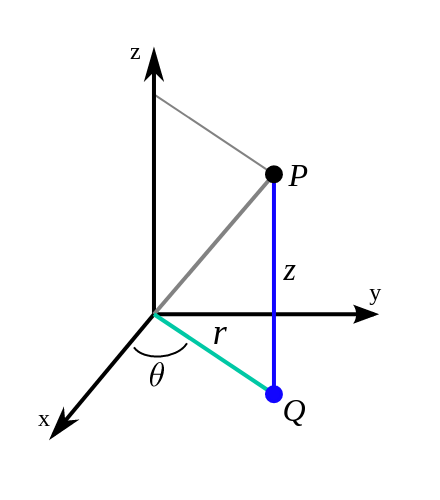
\includegraphics[width=0.5\textwidth]{lambda_theta_cyl_coor.png}
    \end{center}
    \caption{
        $lambda$ is the angle from the equator to the point. $\lambda = \pi/2 - \Theta$, where here $\Theta$ is the well known spherical angle from $z$ axis in spherical coordinate. 
    }\label{fig:def-lambda}
\end{figure}
%%%
Using this assumptions we have
\begin{equation}
    \frac{1}{\rho}\frac{\partial P}{\partial R} = -\frac{\partial \Phi}{\partial R} + \Omega^2 R
\end{equation}
\begin{equation}
    \frac{1}{\rho}\frac{\partial P}{\partial z} = -\frac{\partial \Phi}{\partial z}
\end{equation}
We use gamma equation of state as describe in FLASH code.
\begin{equation}\label{eq:rho-P}
    \gamma_1=\frac{\rho}{P}\frac{\partial P}{\partial \rho} \qquad \mathrm{GAMC\_VAR}
\end{equation}
\begin{equation}\label{eq:gamma_4}
    \gamma_4=1+\frac{P}{\rho\epsilon} \qquad \mathrm{GAME\_VAR}
\end{equation}
for ideal gas $\gamma_1=\gamma_4=\gamma$ and $P=(\gamma-1)\rho\epsilon$.
Where $\epsilon$ is the gas specific internal energy.
The ideal gas equation of state is:
\begin{equation}\label{eq:P-T}
    P=\frac{N_a k}{\bar{A}}\rho T
\end{equation}
Where $N_a$ is avogadro number, $k$ is Boltzmann constant and $\bar A$ is the average atomic mass.
\begin{equation}
    \frac{1}{\bar{A}} = \sum_i\frac{x_i}{A_i} 
\end{equation}
Where $A_i$ is the atomic weight of the species and $x_i$ is the mass fraction of species $i$.
Also it worth mention that radiation will add $P=aT^4/3$ where $a=4\sigma/c$ is the radiation constant and $\sigma$ is Stefan-Boltzmann constant with $\epsilon_{rad}=3P_{rad}/\rho$. The radiation force needed to be added to the momentum equation is 
\begin{equation}
    F_{rad}=-\frac{c}{\kappa\rho}\vec\nabla P_{rad}
\end{equation}
We will first solve eq. \ref{eq:rho-P} to get explicit relation between the density and pressure.
Then we will discuss the angular velocity we use the get thick disk.
And finally we will solve for the density and specific energy to get the initial solution we use in the simulation and described the scheme we use the initialized the simulation.
\begin{equation}
    \frac{\rho}{P}\frac{\partial P}{\partial \rho} = \gamma
\end{equation}
\begin{equation}
    \frac{\rho}{P}\frac{d P}{d \rho} = \gamma
\end{equation}
\begin{equation}
    \frac{d P}{P} = \gamma \frac{d\rho}{\rho}
\end{equation}
\begin{equation}
    d \ln{P} = \gamma d \ln\rho
\end{equation}
\begin{equation}
    d \ln{P} = d \ln\rho^\gamma
\end{equation}
So we get
\begin{equation}
    P=const \rho^\gamma
\end{equation}
and from the initial condition 
\begin{equation}
    P_0=const \rho_0^\gamma
\end{equation}
we get
\begin{equation}
    P=\frac{P_0}{\rho_0^\gamma} \rho^\gamma
\end{equation}
We now, in order to continue, need to discuss the angular velocity.
We seek a Keplerian like velocity 
\begin{equation}
    \Omega(R,z) = - \frac{G M_\star e}{\sqrt{R^2+z^2}}
\end{equation}
Where e is the eccentricity of the trajectory.
We also would like to define the thick disk by an angle $\alpha$ so on line defined by the angle the centripetal force is balanced perfectly by the gravitational potential.
Below this line the matter is confined by gravity and outside this line the matter is unconfined i.e. the centripetal force is bigger then the gravitational force.
This led to constrain on the $\Omega$ as describe in figure \ref{fig:centripect-force}   
%%%
\begin{figure}[ht!]
    \begin{center}
        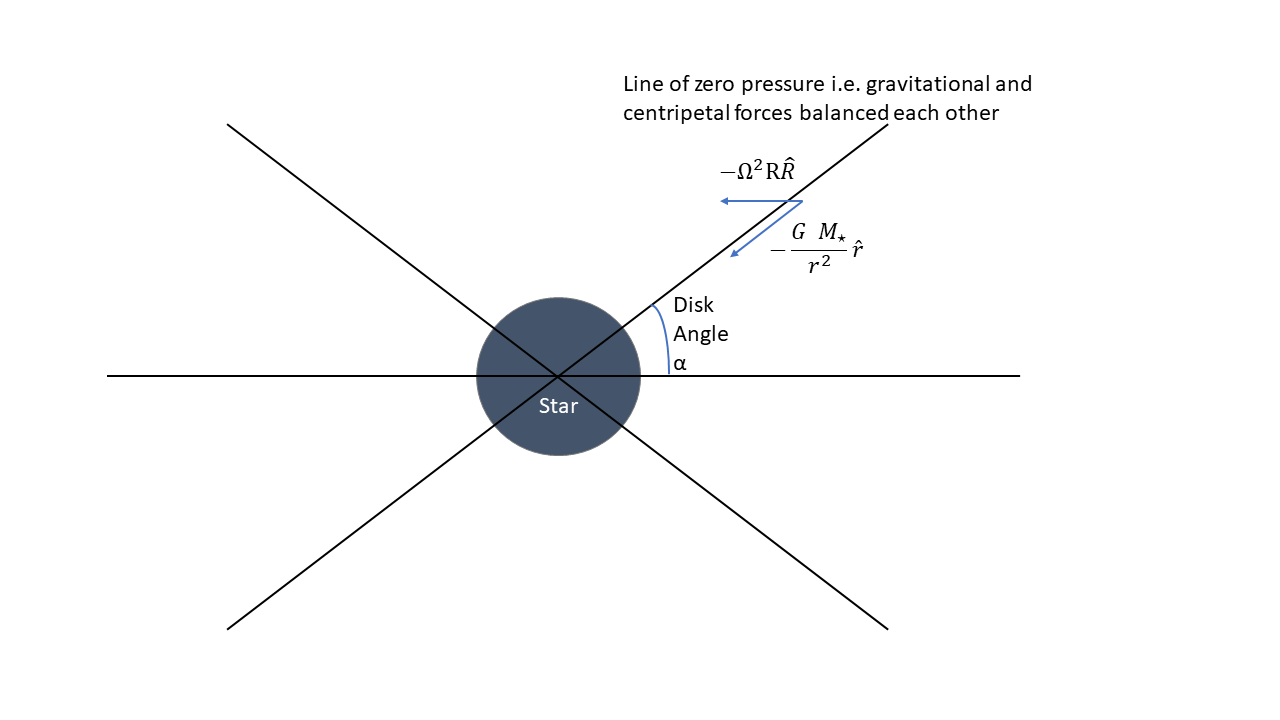
\includegraphics[width=1.0\textwidth]{centripect-force.png}
    \end{center}
    \caption{
        The border line of the thick disk is the line where the gravitational force is balanced by the centripetal force. This line is defined by the disk angle $\alpha$ as $z/R=\tan\alpha$.
    }\label{fig:centripect-force}
\end{figure}
%%%
Now we can finally write the set of equation needed to be solver in order to get the initial solution of the simulation.
\begin{equation}\label{eq:disk_line}
    \frac{G M_\star}{r^2}\cos\alpha = \Omega^2 R, \qquad r^2=R^2+z^2, \qquad z=R\tan\alpha
\end{equation}
\begin{equation}\label{eq:rho-z}
    \frac{1}{\rho}\frac{d P}{d \rho}\frac{\partial \rho}{\partial z} = -\frac{\partial \Phi}{\partial z}
\end{equation}
\begin{equation}\label{eq:rho-R}
    \frac{1}{\rho}\frac{d P}{d \rho}\frac{\partial \rho}{\partial R} = -\frac{\partial \Phi}{\partial R} + \Omega^2 R
\end{equation}
\begin{equation}
    P=\frac{P_0}{\rho_0^\gamma}\rho^\gamma ~;\qquad \Phi=-\frac{G M_\star}{\sqrt{R^2+z^2}} 
\end{equation}
From eq. \ref{eq:rho-z} we get
\begin{equation}
    \frac{1}{\rho}\frac{P_0}{\rho_0^\gamma}\gamma\rho^{\gamma-1}\frac{\partial \rho}{\partial z} = - \frac{\partial \Phi}{\partial z}
\end{equation}
\begin{equation}
    \frac{P_0}{\rho_0^\gamma}\frac{\gamma}{\gamma-1}\rho^{\gamma-1}=-\Phi
\end{equation}
And solving eq. \ref{eq:rho-R}
\begin{equation}
    \frac{P_0}{\rho_0^\gamma}\frac{\gamma}{\gamma-1}\rho^{\gamma-1}=-\Phi + \int \Omega^2 R dR
\end{equation}
where the last term need to be a function of $R$ only.
Using eq. \ref{eq:disk_line} the last term become
\begin{equation}
    \int \frac{G M_\star \cos\alpha}{R^2+(R\tan\alpha)^2} dR = 
    \int \frac{G M_\star}{R^2}\cos^3\alpha dR =
    -\frac{G M_\star}{R}\cos^3\alpha
\end{equation}
This give
\begin{equation}
    \rho^{\gamma-1}=\frac{\rho_0^\gamma}{P_0}\frac{\gamma-1}{\gamma}\left( -\Phi -\frac{G M_\star}{R}\cos^3\alpha \right) 
\end{equation}
And after substituting the gravitational potential we get
\begin{equation}\label{eq:rho_solution}
    \boxed{
        \rho^{\gamma-1}=\frac{\rho_0^\gamma}{P_0}\frac{\gamma-1}{\gamma} G M_\star \left( \frac{1}{\sqrt{r^2+z^2}} -\frac{\cos^3\alpha}{R} \right)
    }
\end{equation}
The parameters of the problem is $\rho_0$ and the disk angle $\alpha$. This two parameters determine exactly the functionality and values of all other quantities.
$\rho_0$ is the density at the end of the star i.e. at $r=r_\star$.
We now describe the initialization scheme.
\begin{itemize}
    \item Setting $\gamma=5/3$ and $\alpha\sim 30^\circ$.
    \item Calculate $\rho$ using eq. \ref{eq:rho_solution}
    \item Calculate $P$ using $P=(P_0/\rho_0^\gamma) ~ \rho^\gamma$. We calculate $P_0$ using eq. \ref{eq:rho_solution} where we assume $z=0$ and $R=r_\star$. So the left hand term is $\rho_0^{\gamma-1}$. And we get 
    \begin{equation}
        P_0=\rho_0\frac{\gamma-1}{\gamma}\frac{G M_\star}{r_\star}\left(1-\cos^3\alpha\right)
    \end{equation}
    \item Calculate the specific energy $\epsilon$.
    \begin{equation}
        \epsilon = \frac{P}{(\gamma-1)\rho}=\frac{P_0}{\rho_0^\gamma}\frac{\rho^{\gamma-1}}{\gamma-1} = \frac{1}{\gamma} G M_\star \left( \frac{1}{\sqrt{r^2+z^2}} -\frac{\cos^3\alpha}{R} \right)
    \end{equation}
    \item Setting the velocity $u_x,~u_y,~u_z$ to
    \begin{equation}
        u_z=0, \qquad u_x=-\Omega R \sin \theta, \qquad u_y= \Omega R \cos\theta
    \end{equation}
    Where 
    \begin{equation}
        \Omega=\sqrt{\frac{G M_\star}{R^3}\cos^3\alpha}
    \end{equation}
    \item Calculate the temperature using eq. \ref{eq:gamma_4} and eq. \ref{eq:P-T}
    \begin{equation}
        T=\frac{(\gamma-1)\epsilon \bar{A}}{N_a k} = \frac{\epsilon(\gamma-1)\mu m_H}{k}
    \end{equation}
    where $\mu \sim 0.617$ is the mean molecular weight for solar composition $ 1/\mu = N_a m_H /\bar A $.
    \item Set the specific radiation energy $\epsilon_{rad}=3P_{rad}/\rho=a T^4/\rho$ where $P_{rad}=a T^4/3$.
    \item Set in the region $r<r_\star$ the velocities to zero. This led to the simple solution 
    \begin{equation}
        \rho^{\gamma-1}=\frac{\rho_0^\gamma}{P_0}\frac{\gamma-1}{\gamma} \frac{G M_\star}{\sqrt{r^2+z^2}}
    \end{equation}
    and set all the relevant quantities accordingly (like temperature, radiation energy and etc.)
\end{itemize}
Also after each time step of simulation calculation we adjust the region $r<r_\star$ to it initial region. 
We notice that as $R\rightarrow0$ the solution for $\rho$ become ill defined as the gravitational potential is much less then the centripetal contribution.
In the region outside the disk ($\lambda>\alpha$ where $\lambda$ is the elevation angle from x-y plane) we can have $1/r < cos^3\alpha/R $ which led to invalid density this of course can not happen in the region inside the disk $\lambda<\alpha$.
To over come this issue we set the density in the region $\lambda>\alpha$ to be 
\begin{equation}\label{eq:rho_outside_disk}
    \rho^{\gamma-1}=\frac{\rho_0^\gamma}{P_0}\frac{\gamma-1}{\gamma} \frac{G M_\star}{r} \left( 1 - \cos^2\alpha \right)
\end{equation}
This suggested solution fix the density to the disk line ($R/r=\cos\alpha$).

%figure of the initial condition
Here we can see the initial setup (fig:\ref{fig:dens-3d-t0},\ref{fig:dens-vel-xy-t0},\ref{fig:dens-xy-t0}).
%%%
\begin{figure}[ht!]
    \begin{center}
        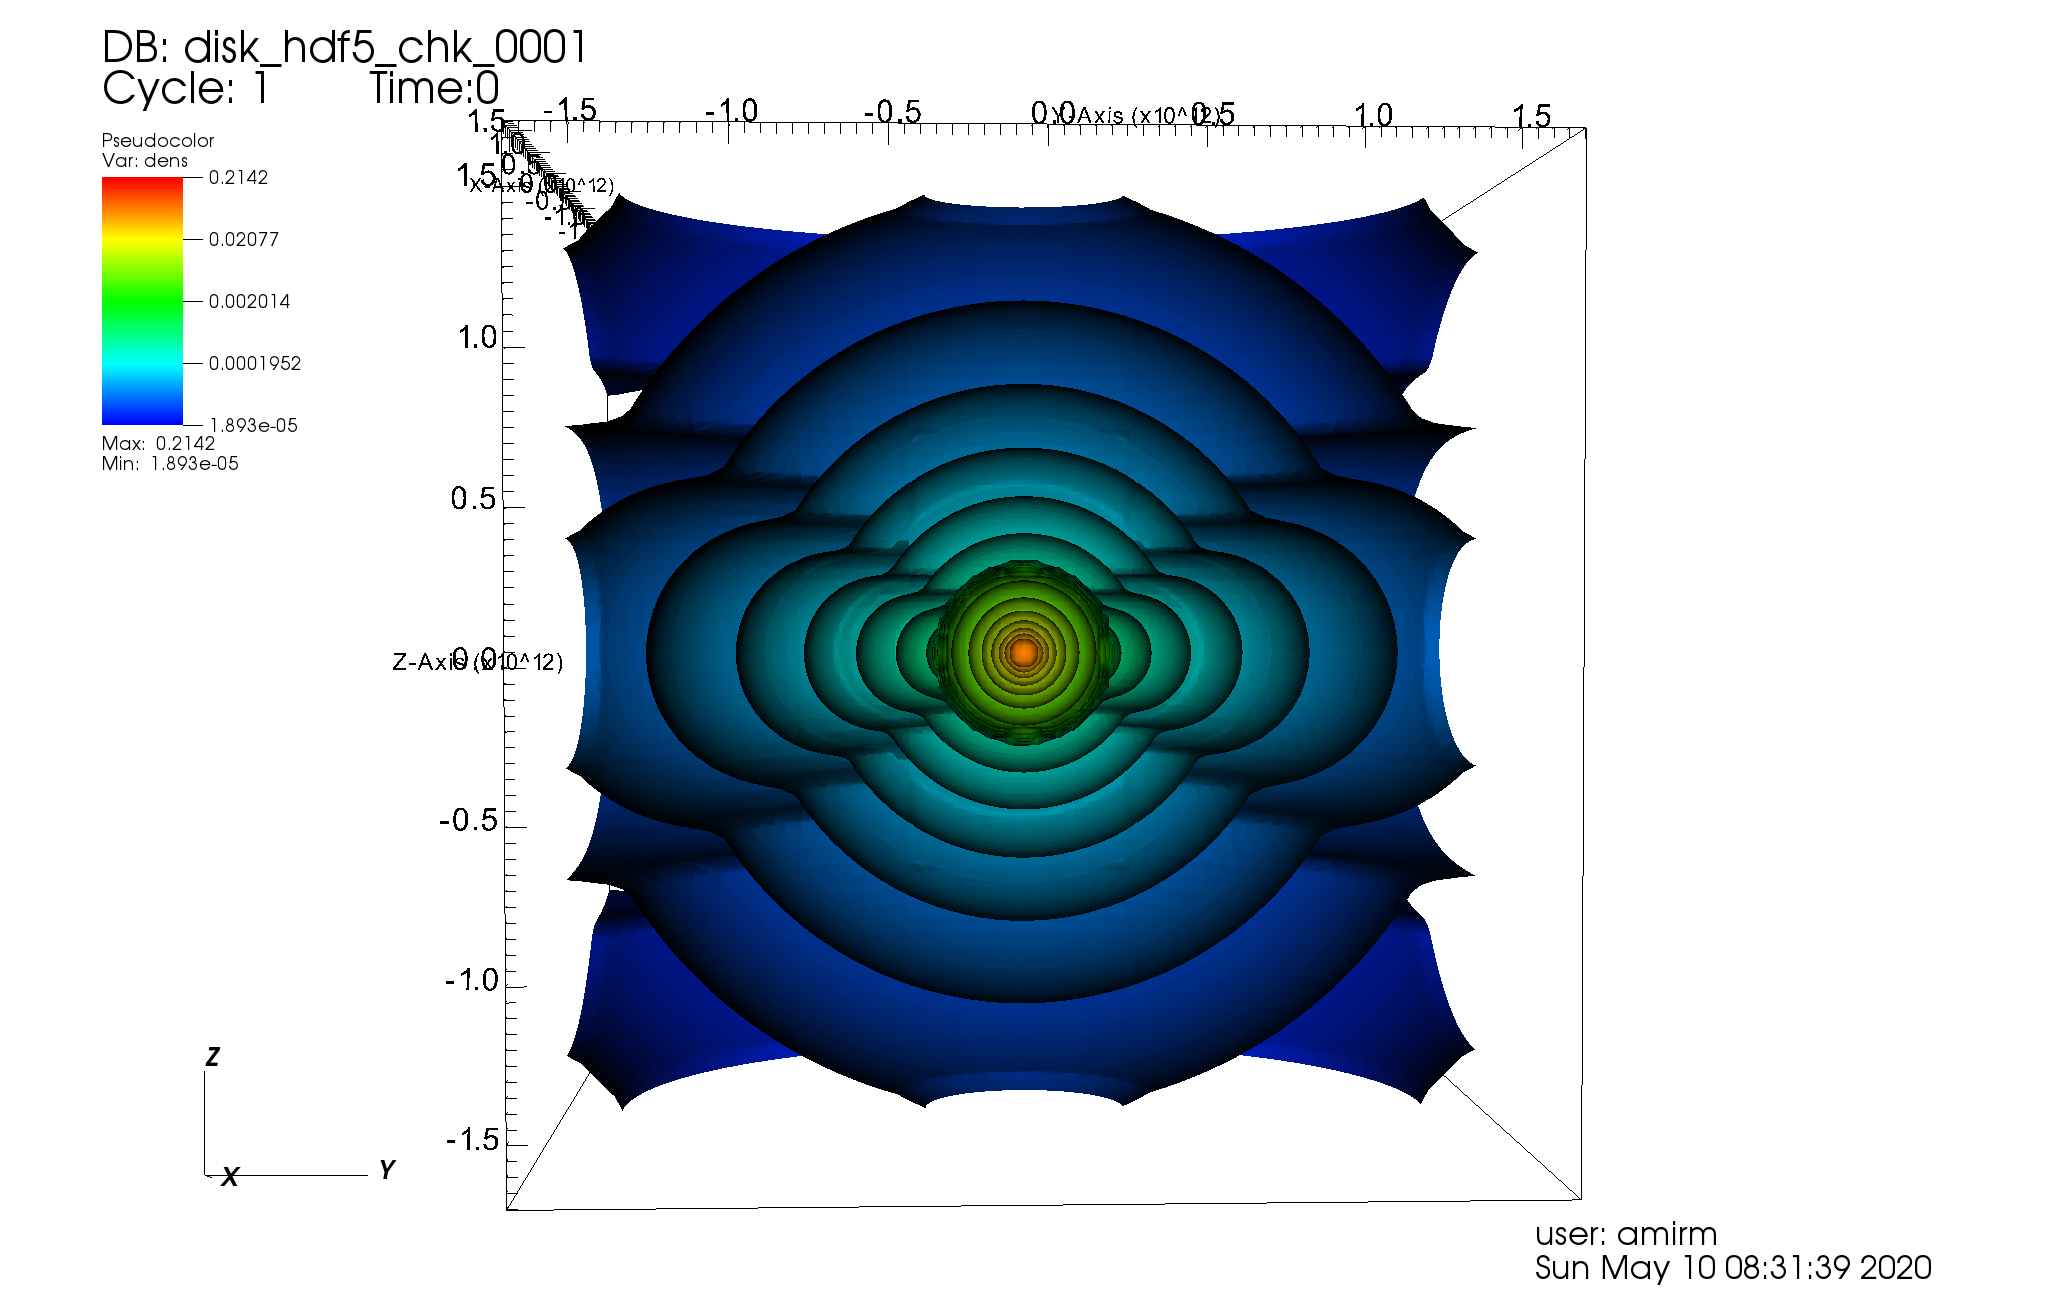
\includegraphics[width=1.0\textwidth]{density_t0_3d.png}
        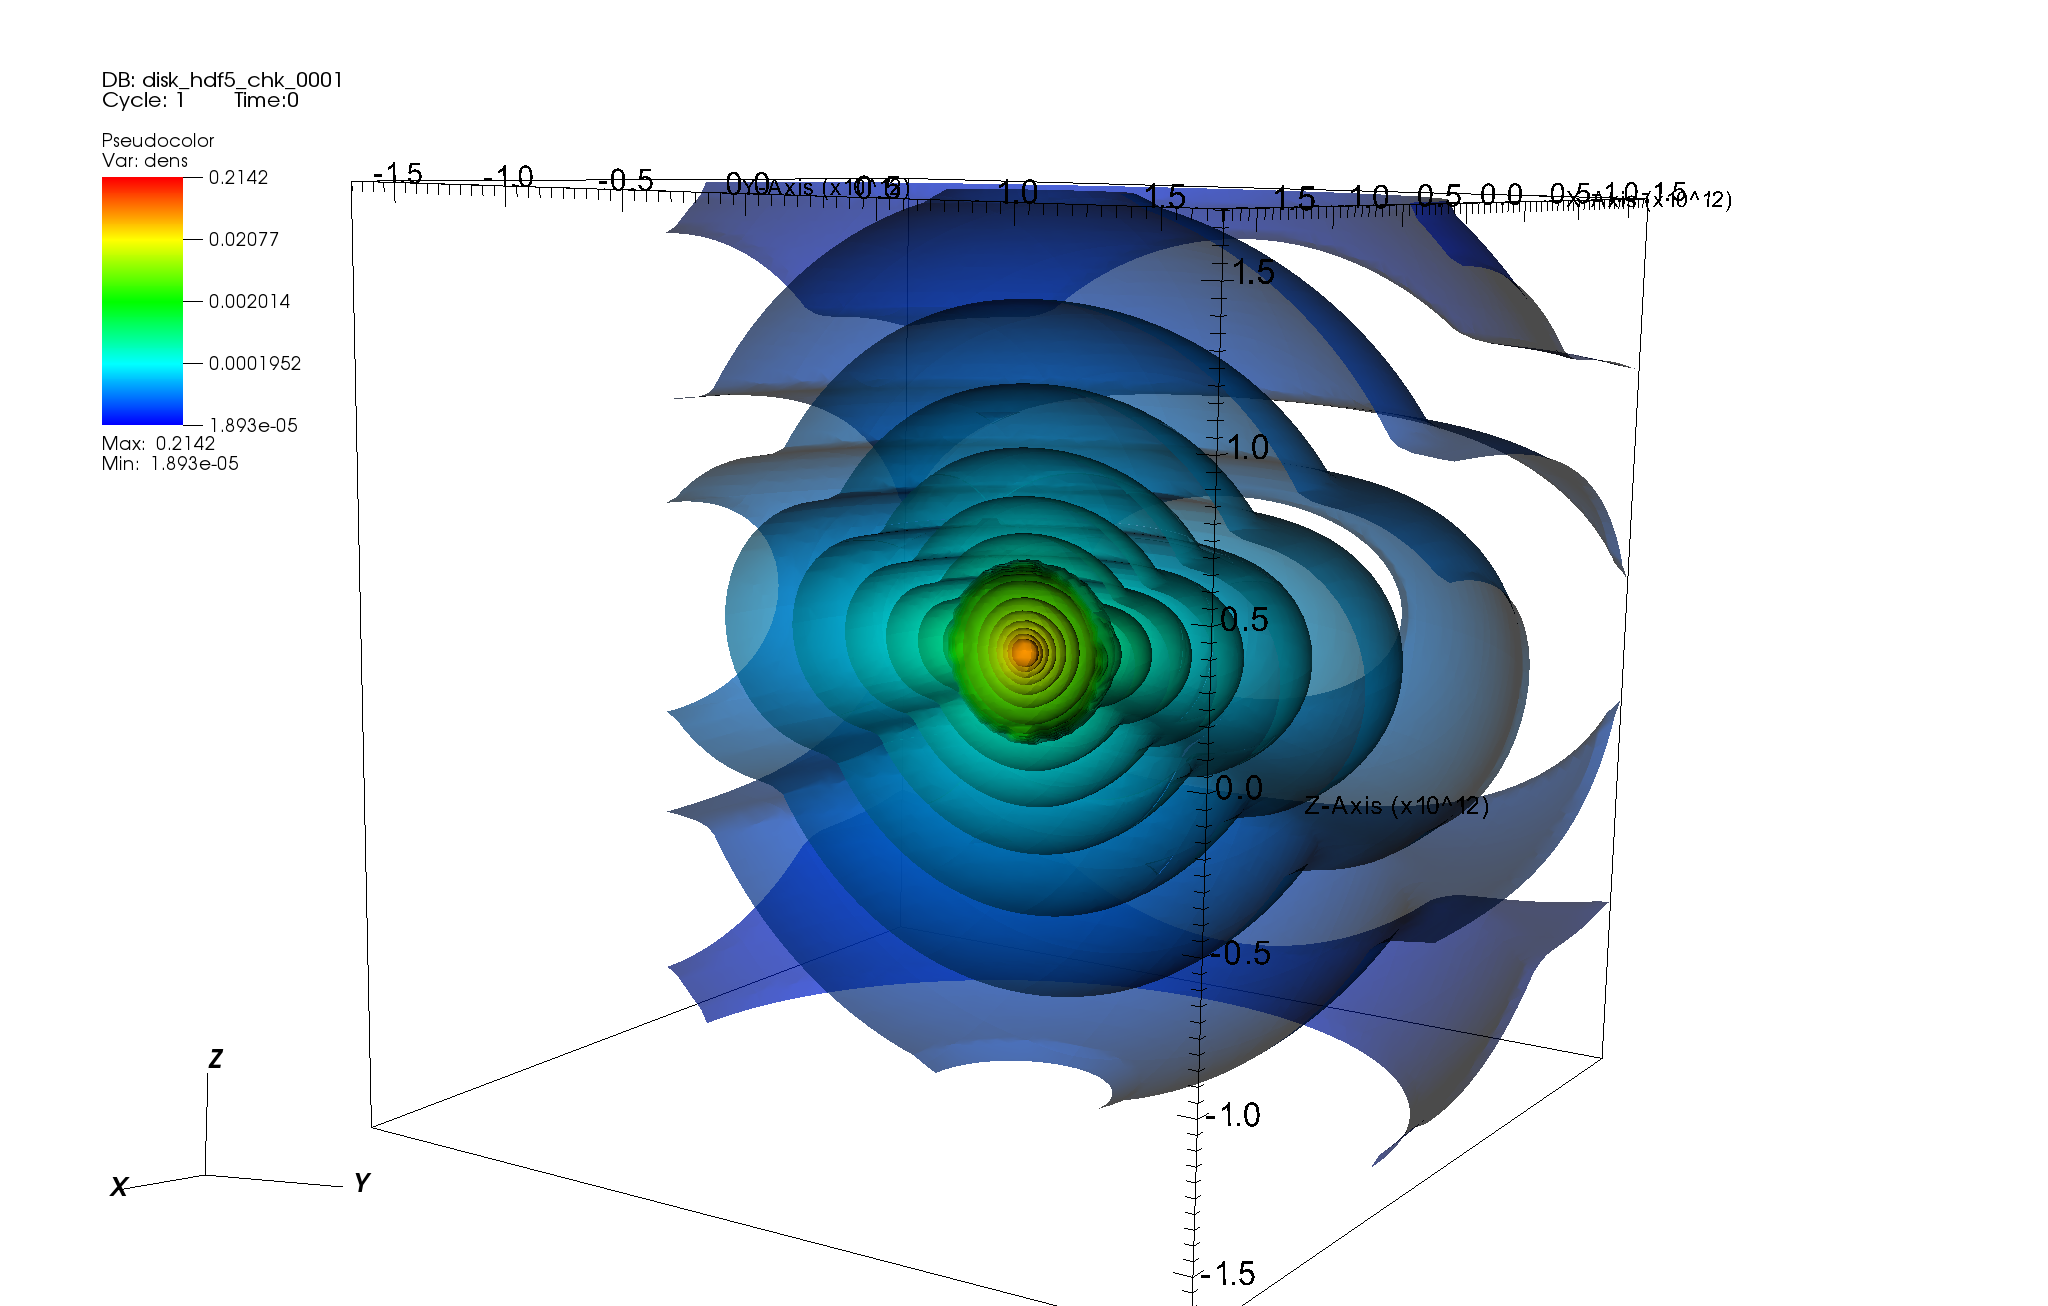
\includegraphics[width=1.0\textwidth]{density_t0_3d_side.png}
    \end{center}
    \caption{
        Density initial solution. 3D isosurface. 
    }\label{fig:dens-3d-t0}
\end{figure}
\begin{figure}[ht!]
    \begin{center}
        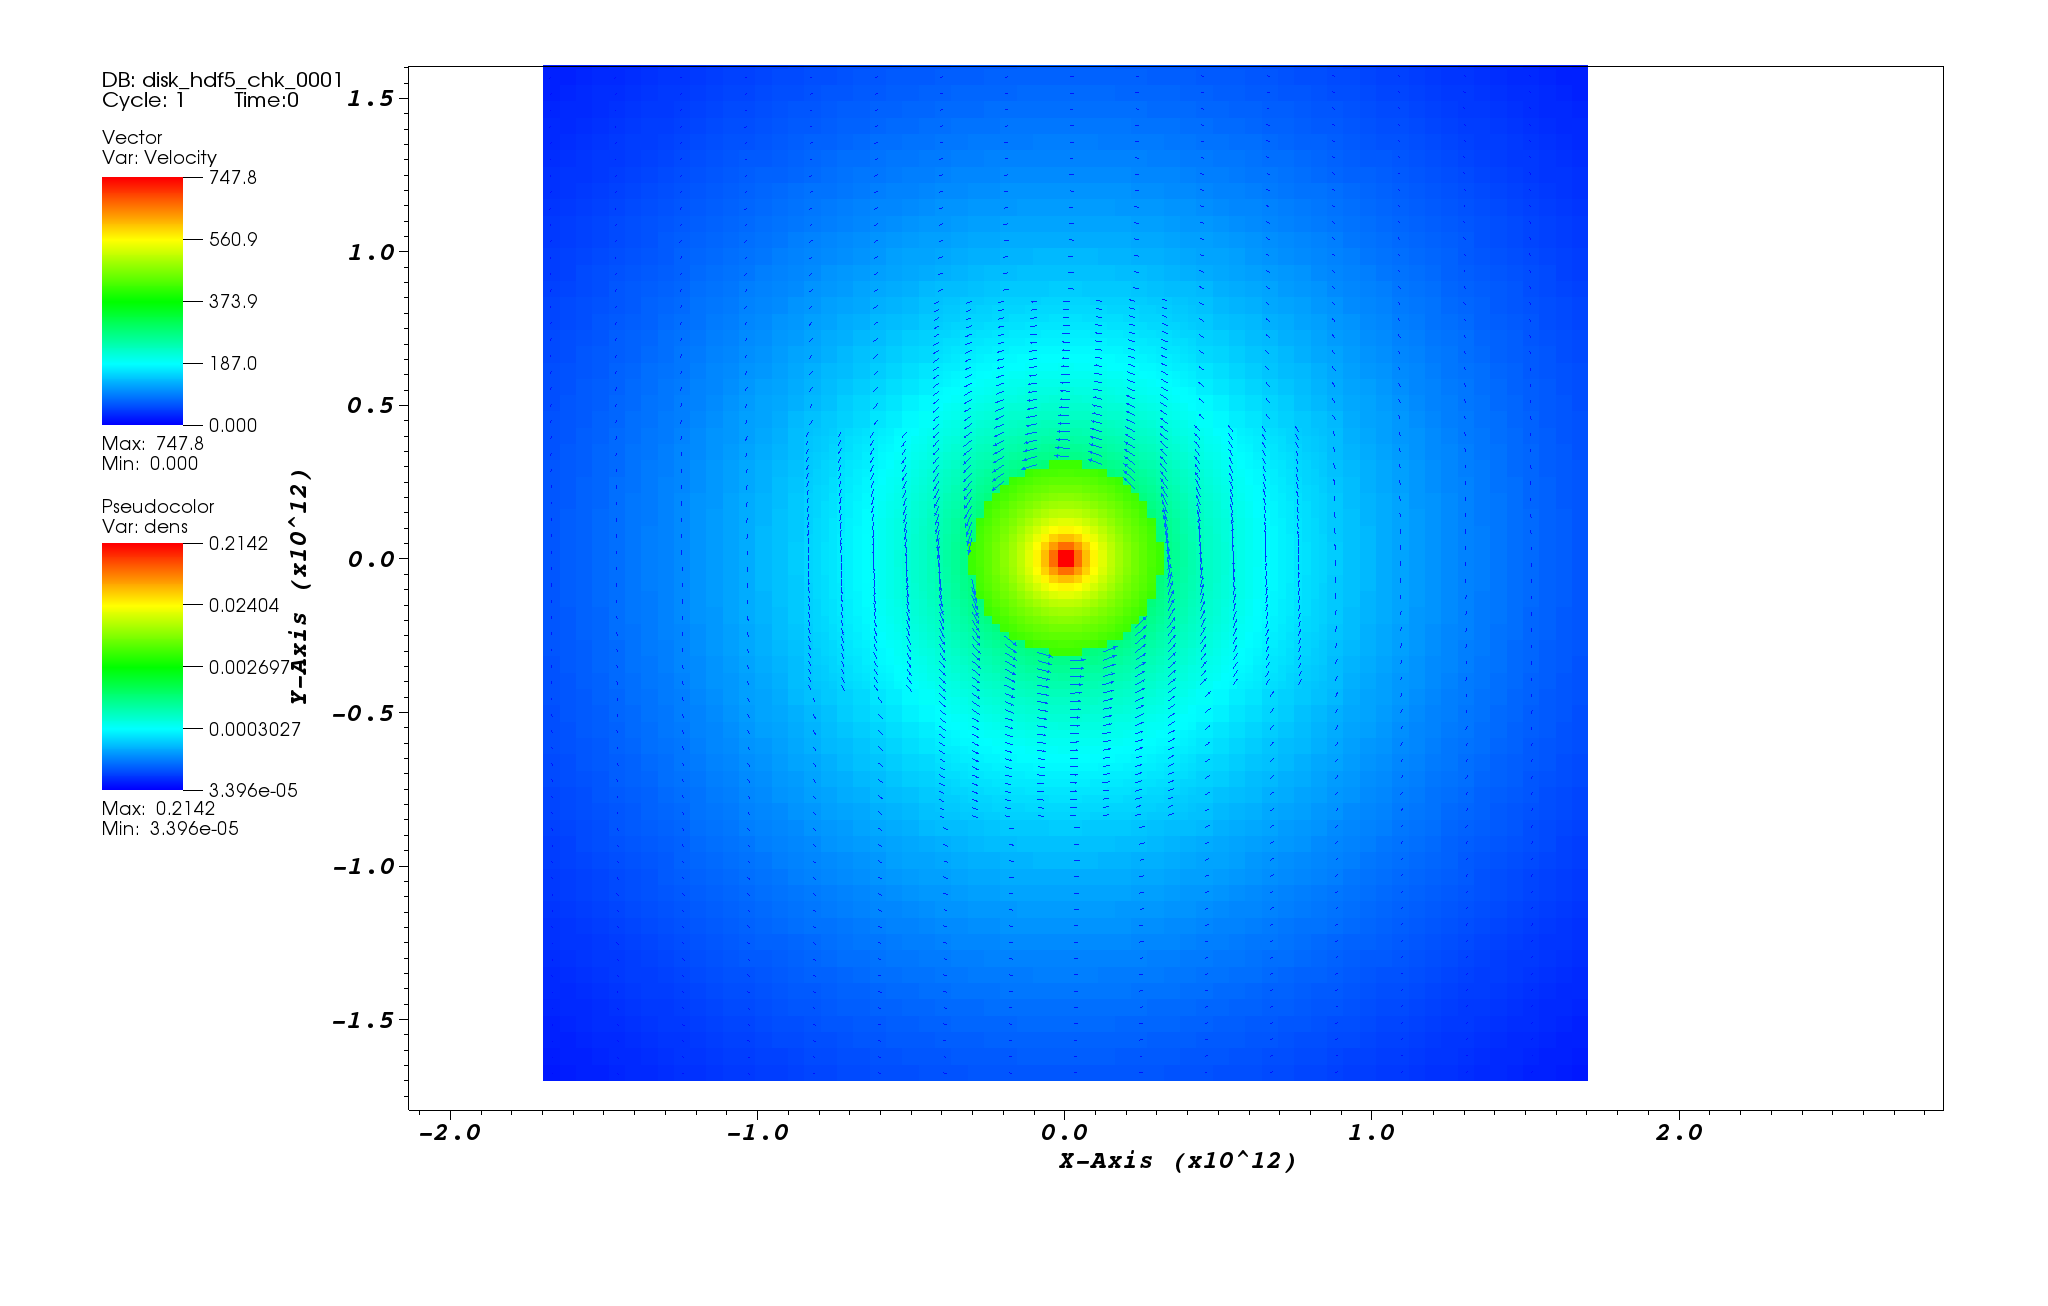
\includegraphics[width=1.0\textwidth]{density-vel-x-y.png}
    \end{center}
    \caption{
        Density and velocity initial condition at the x-y plane. The velocity is Keplerian as expected. 
    }\label{fig:dens-vel-xy-t0}
\end{figure}
\begin{figure}[ht!]
    \begin{center}
        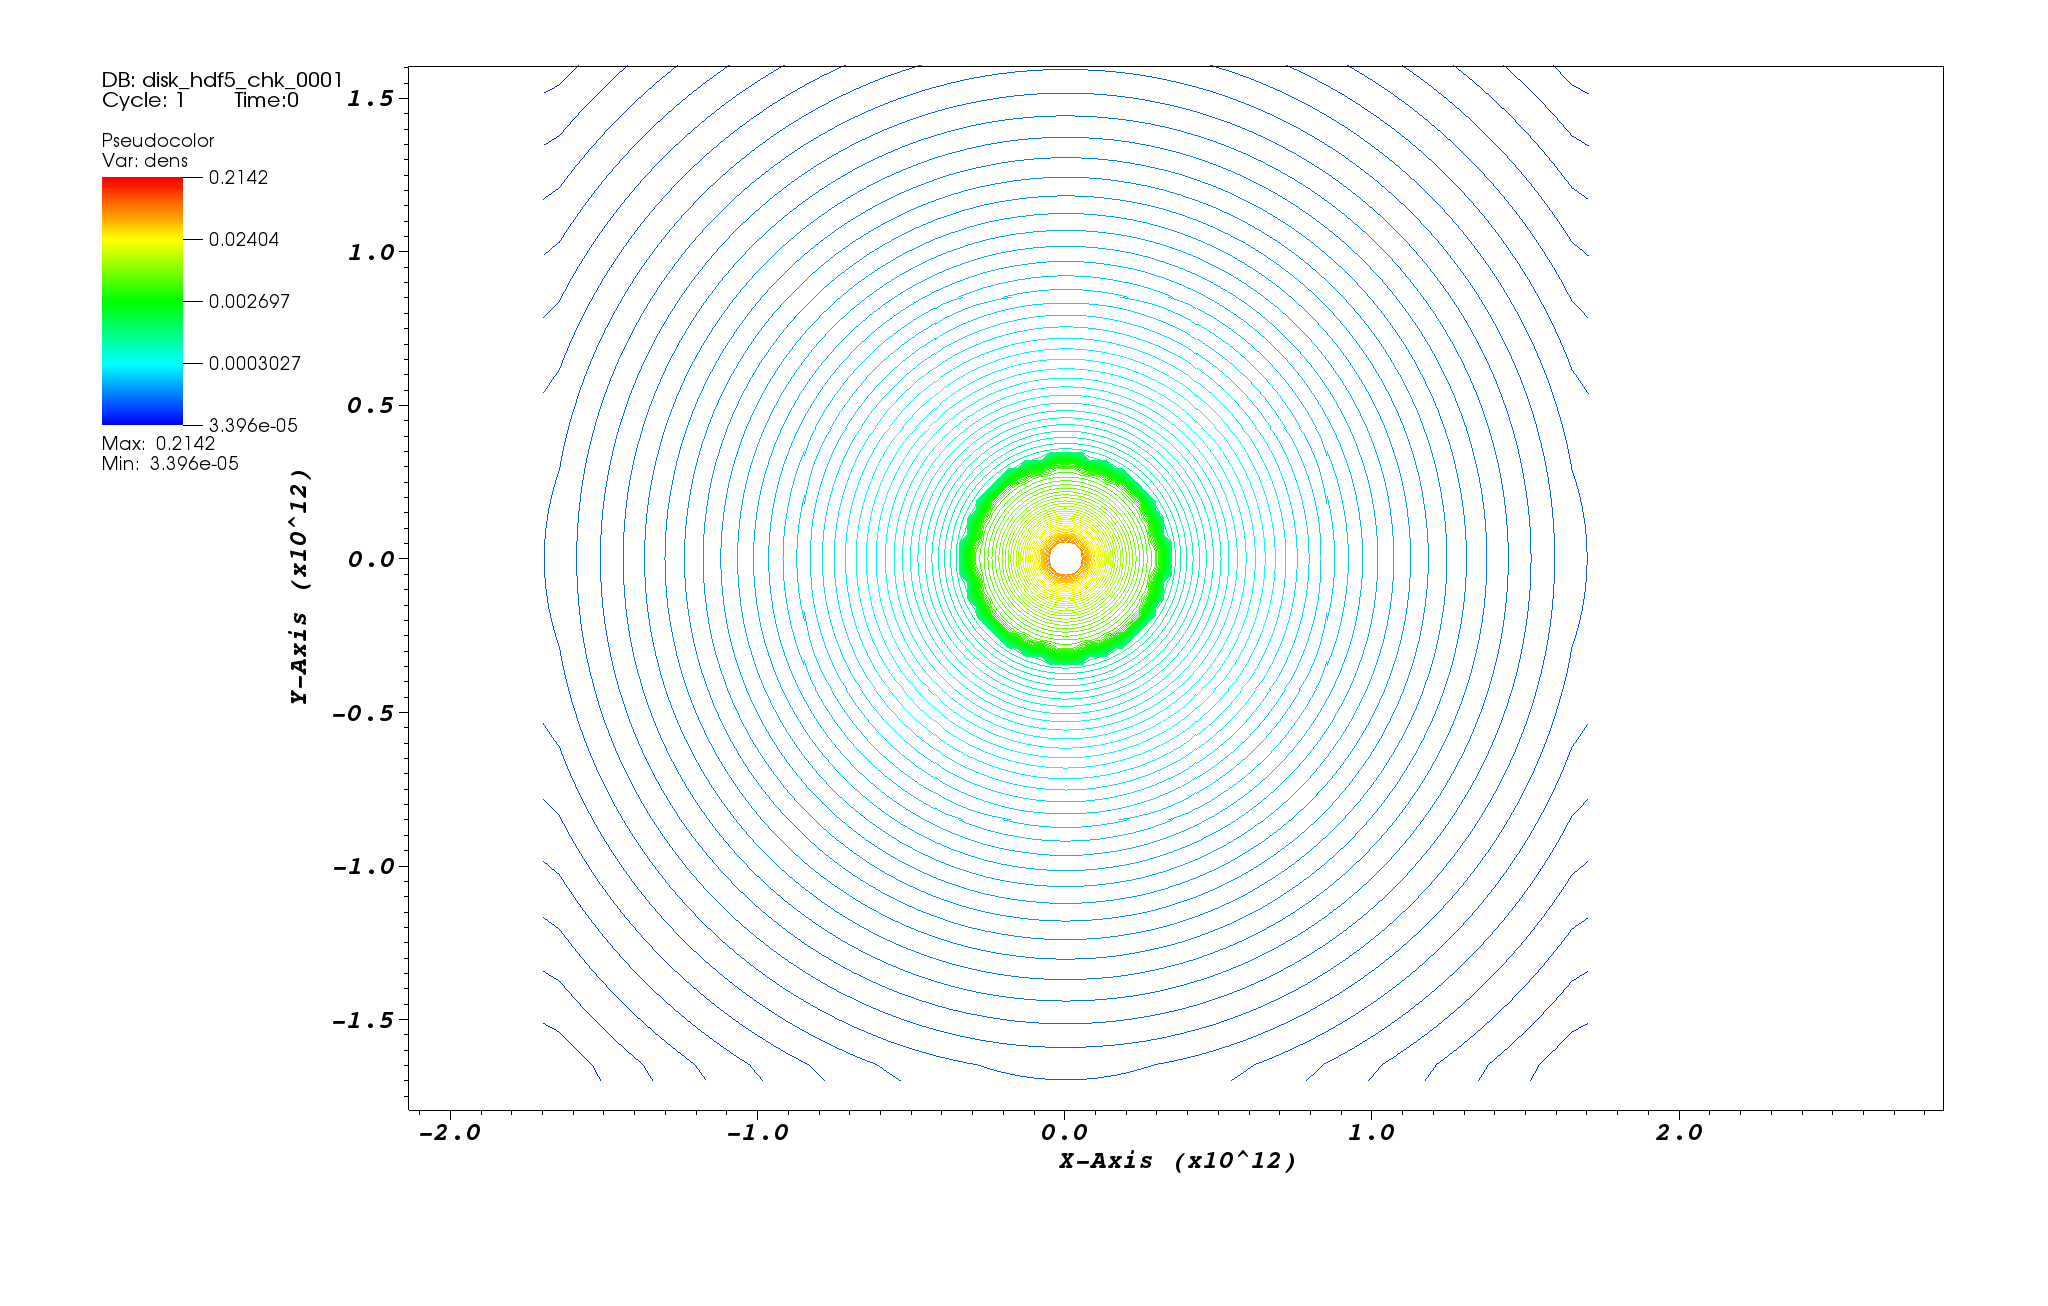
\includegraphics[width=1.0\textwidth]{density-x-y-isosurf-t0.png}
        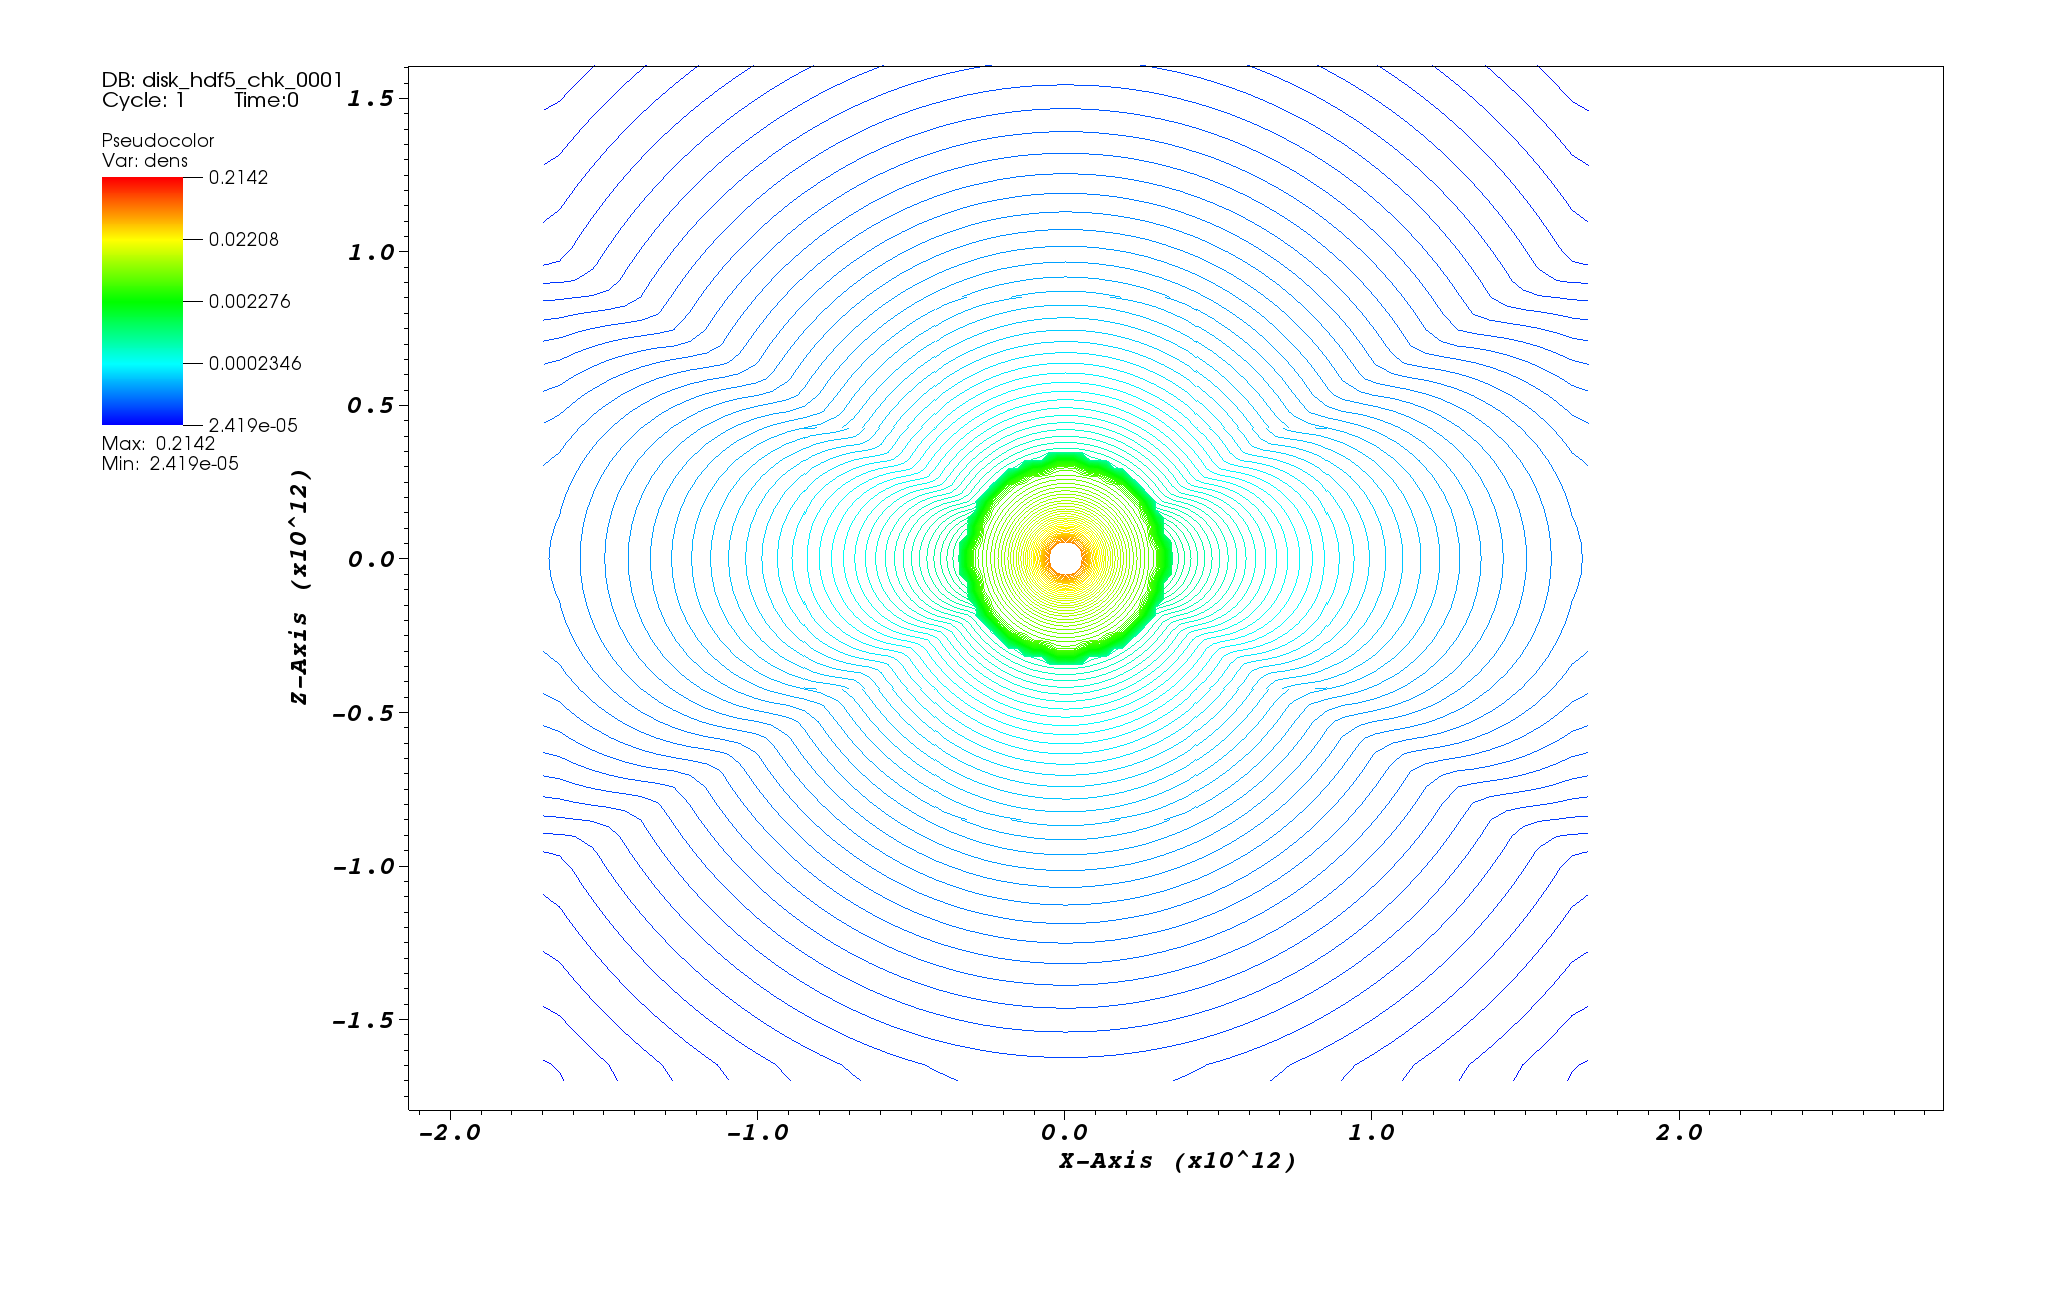
\includegraphics[width=1.0\textwidth]{density-x-z-isosurf-t0.png}
    \end{center}
    \caption{
        The starting density isosurface at the plane (x,y,0) and (x,0,z). 
    }\label{fig:dens-xy-t0}
\end{figure}

%two figure of the result
Here we can see some initial result from compute canada computers.
It was two iteration each of 12 hours run (real life time) fig:\ref{fig:dens-xz-t5-t11},\ref{fig:dens-3d-t5-t11},\ref{fig:dens-vel-xy-t5-t11}.
\begin{figure}[ht!]
    \begin{center}
        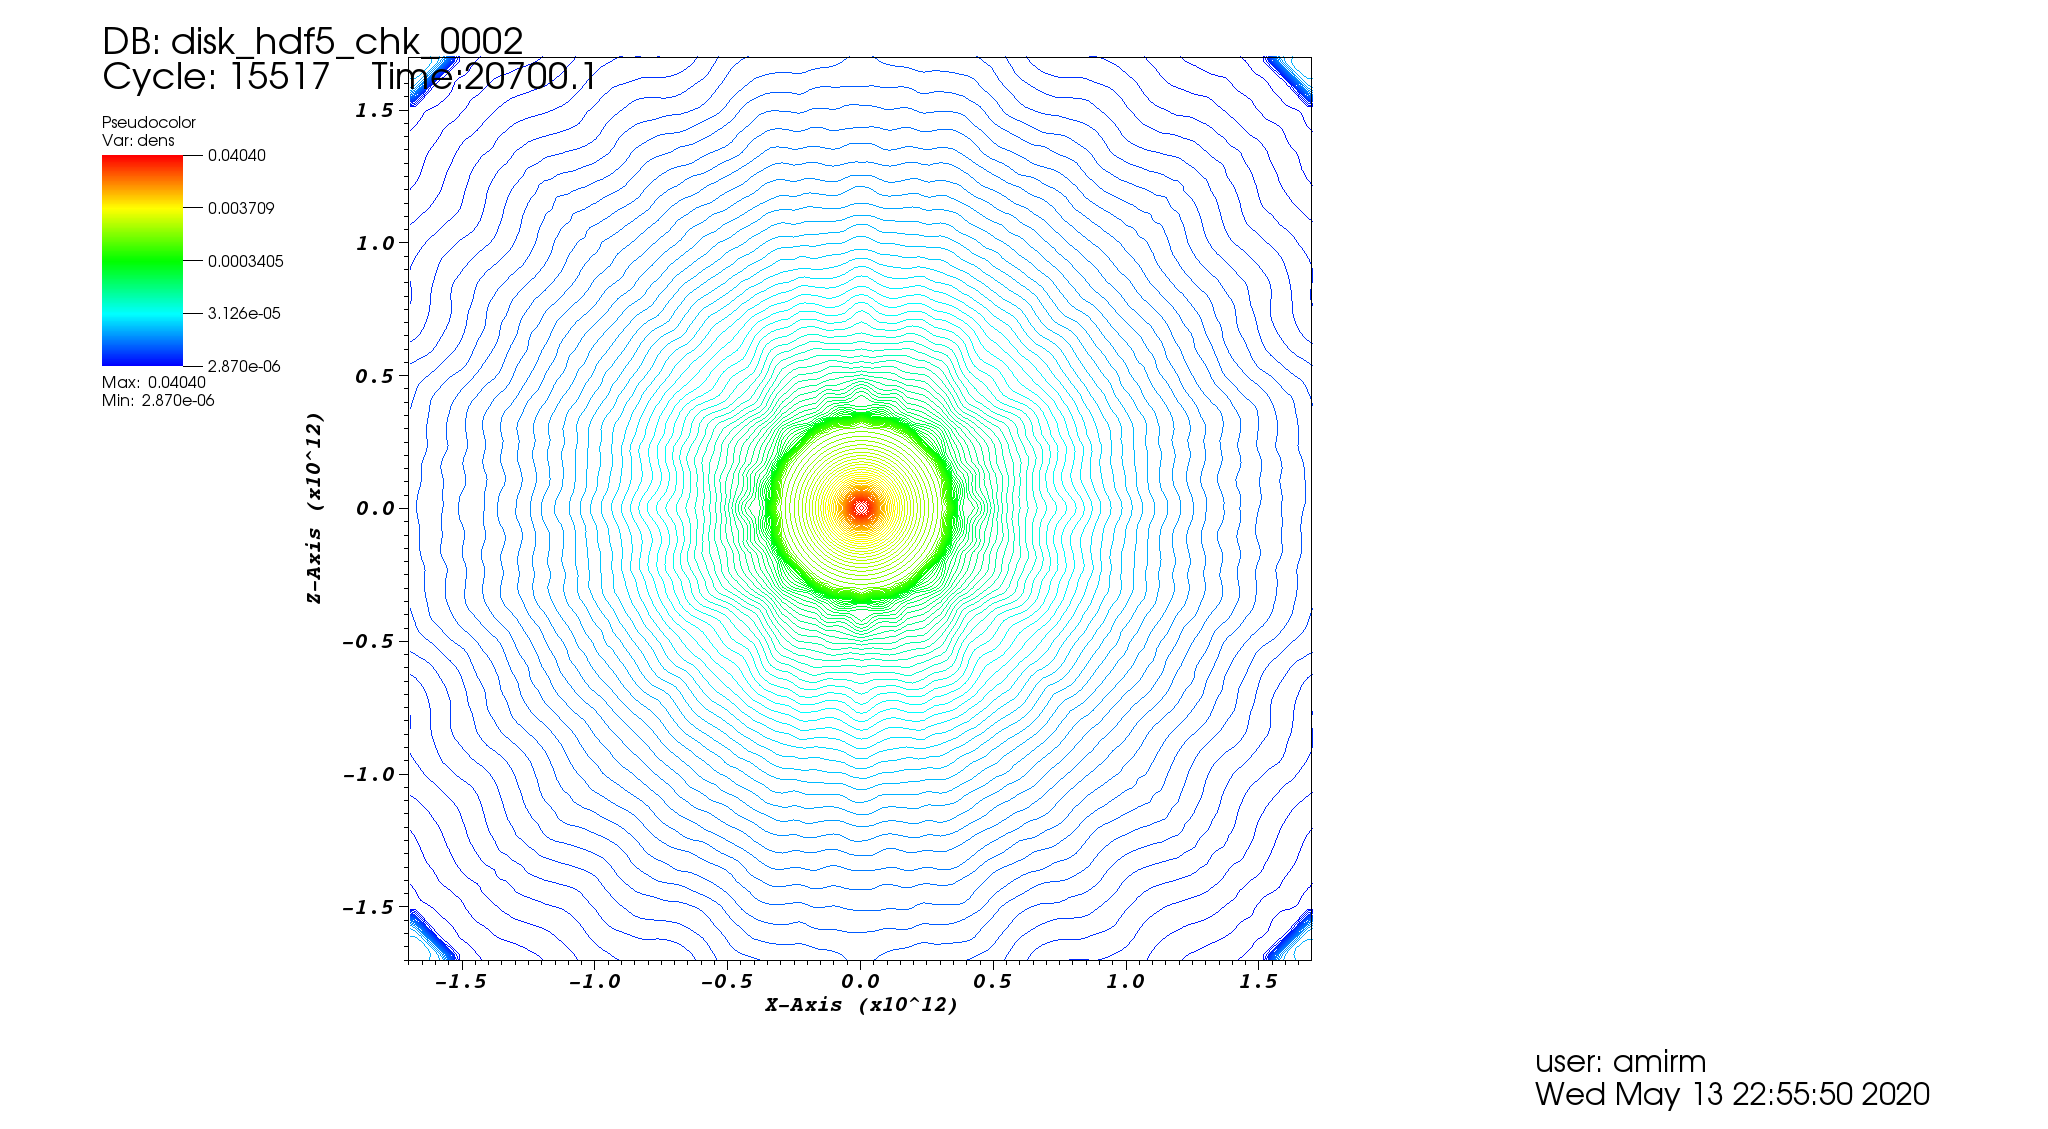
\includegraphics[width=1.0\textwidth]{density-x-z-5-75.png}
        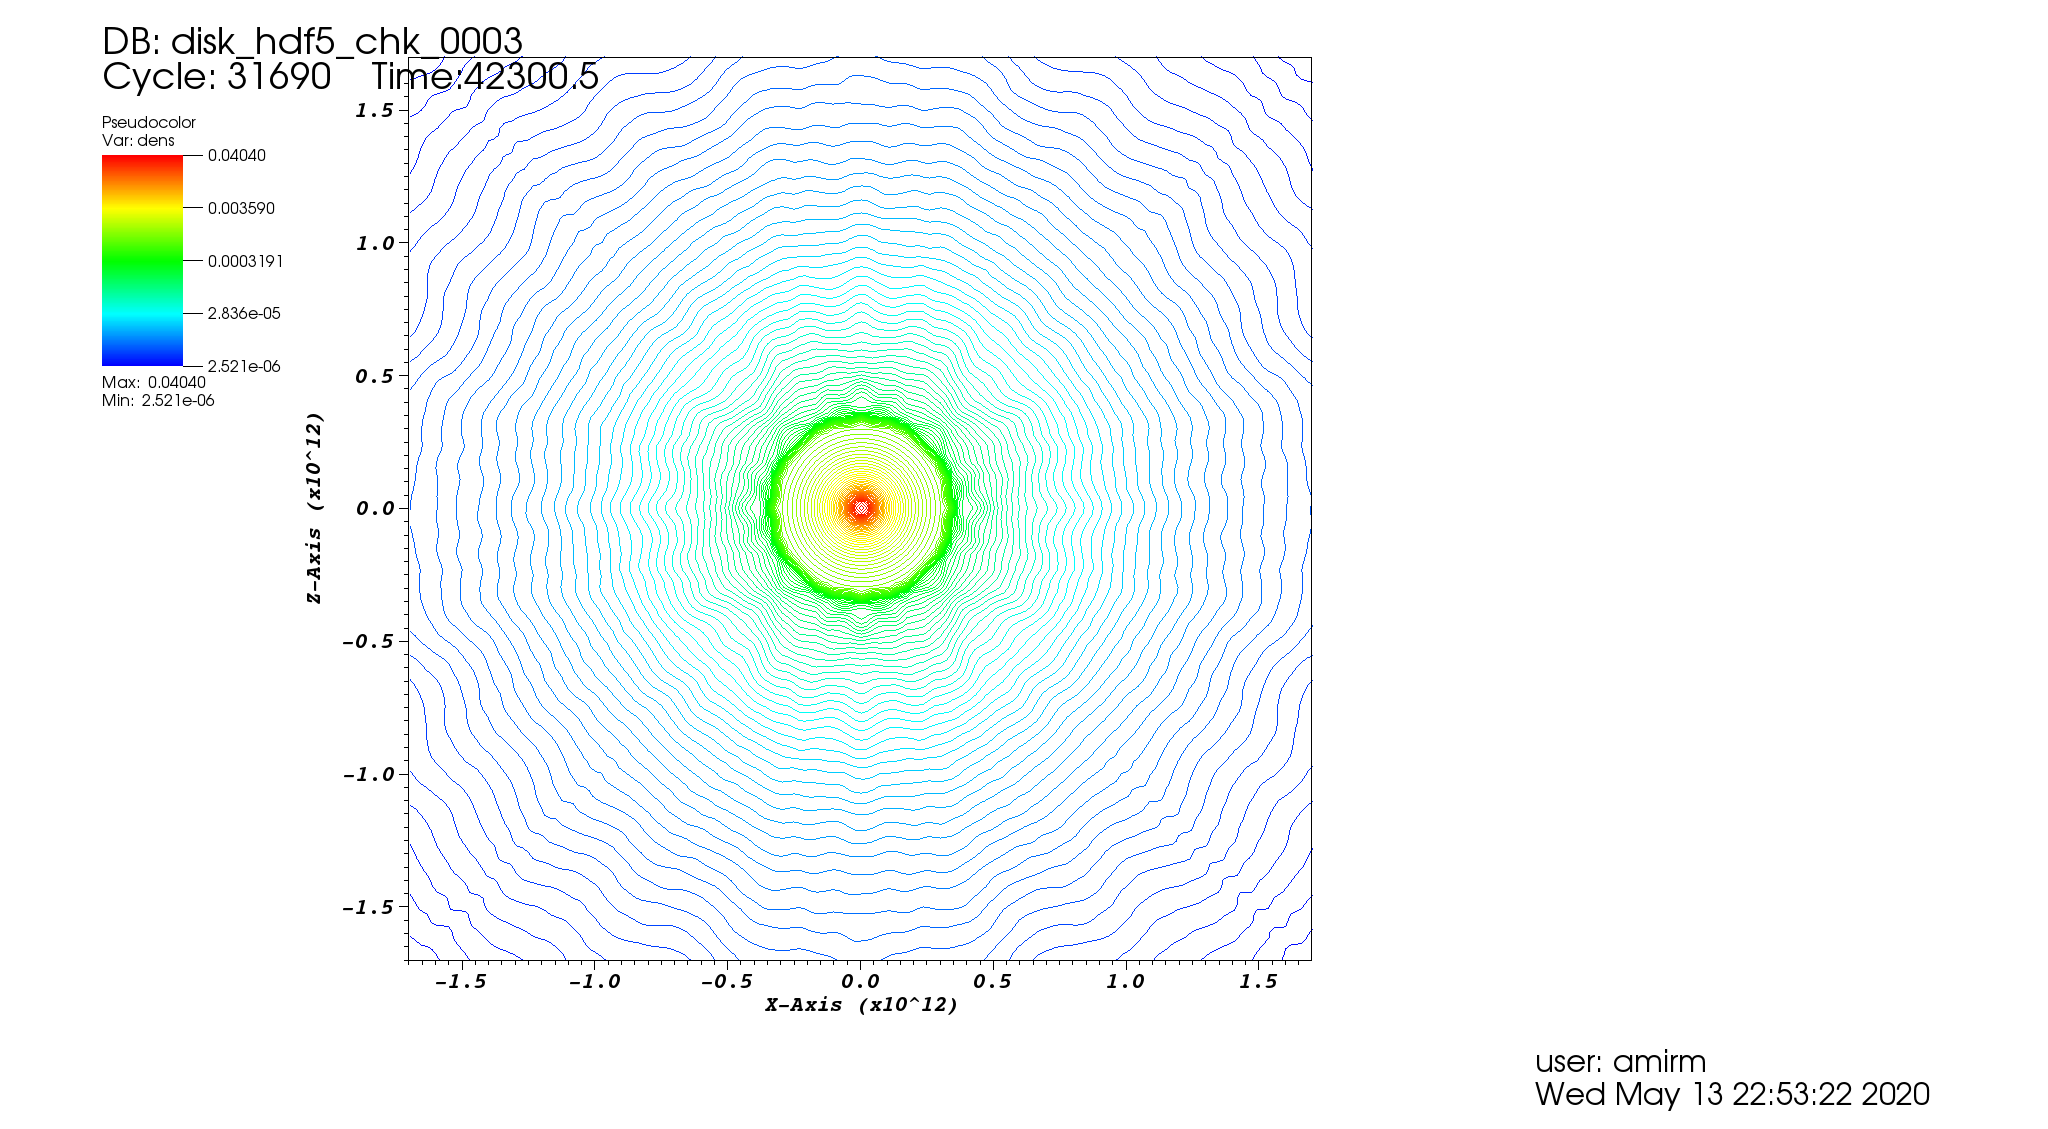
\includegraphics[width=1.0\textwidth]{density-x-z-11-75.png}
    \end{center}
    \caption{
        The density at (x,0,z) plane after 5:45 hours (simulation time) and 11:45 hours (simulation time).
    }\label{fig:dens-xz-t5-t11}
\end{figure}

\begin{figure}[ht!]
    \begin{center}
        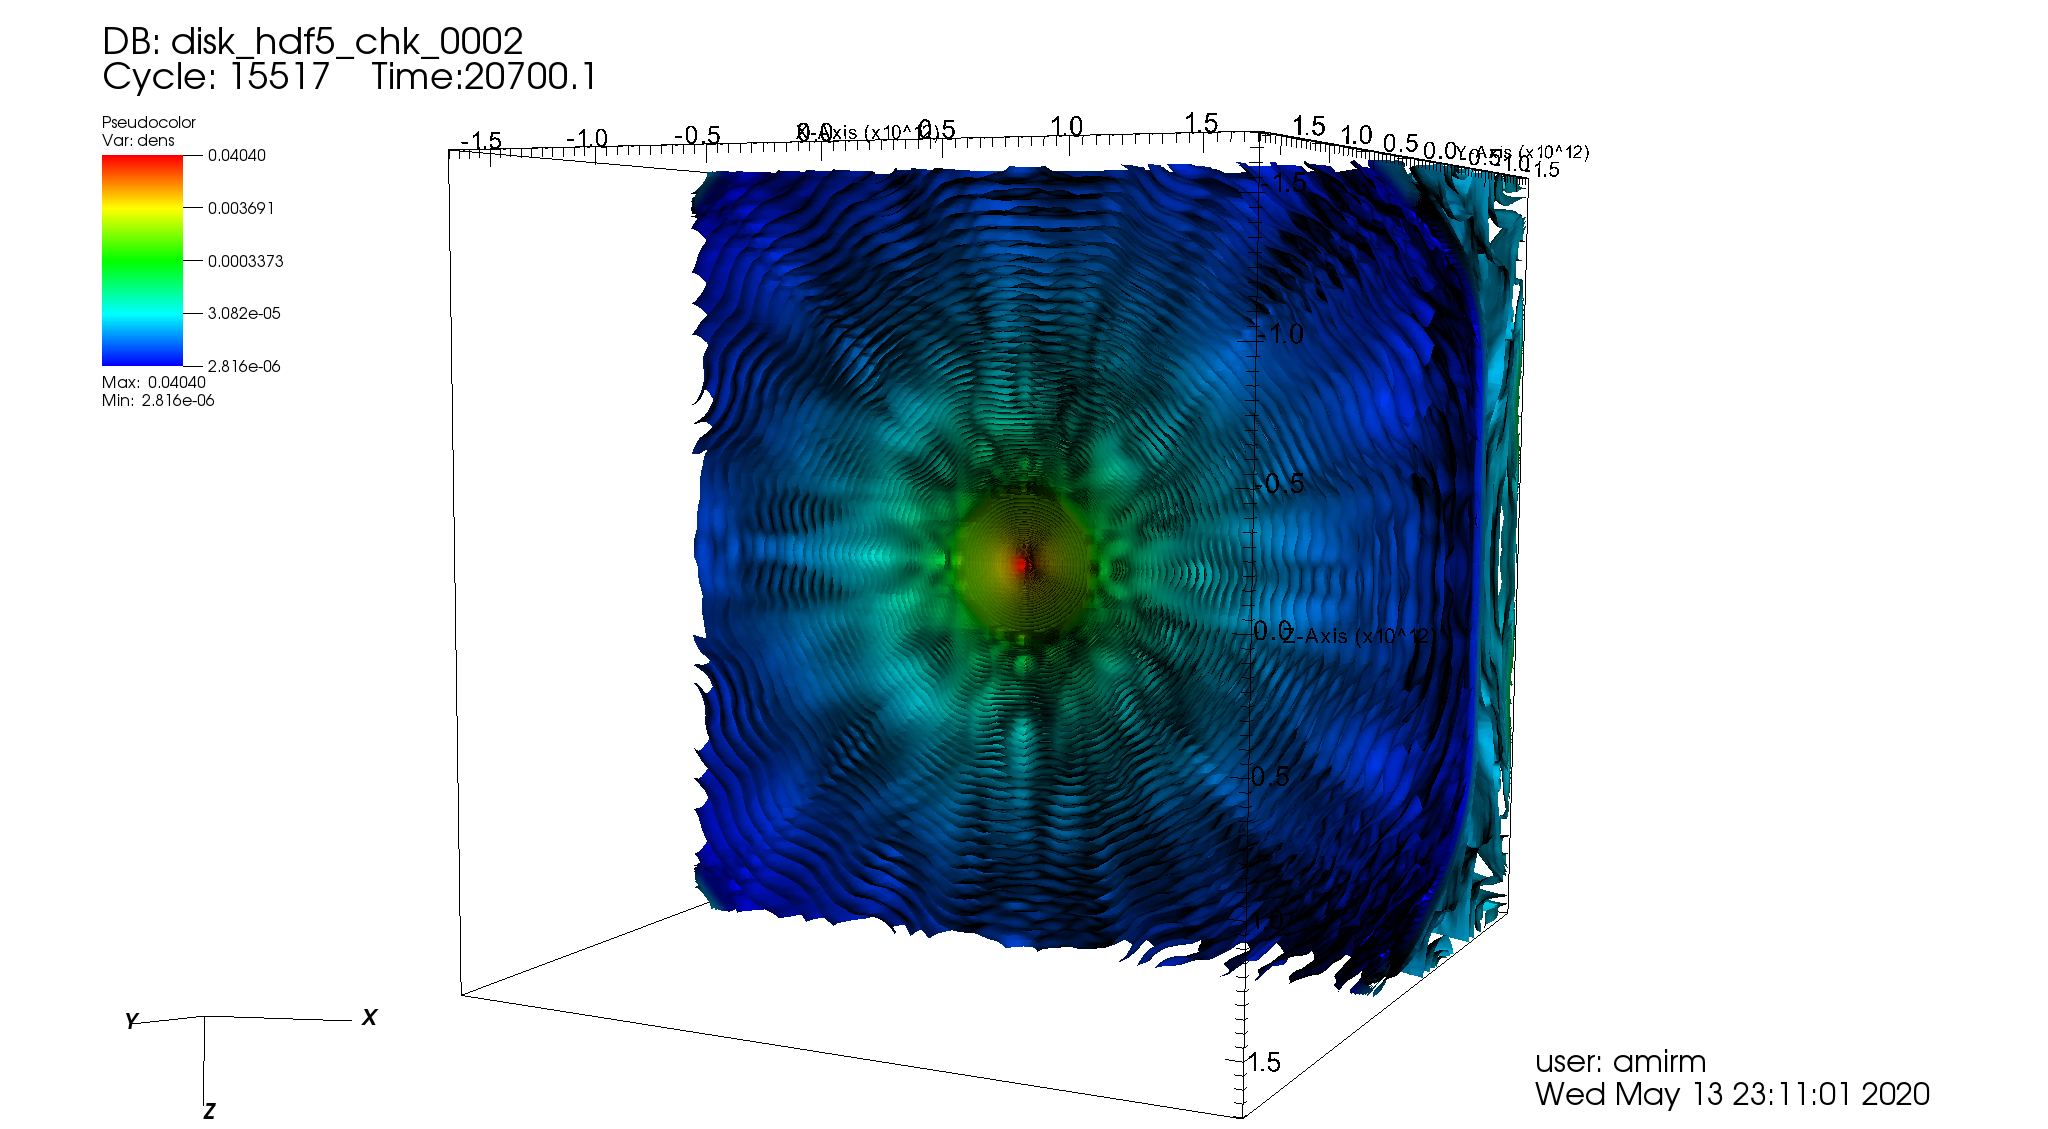
\includegraphics[width=1.0\textwidth]{density-3d-5-75.png}
        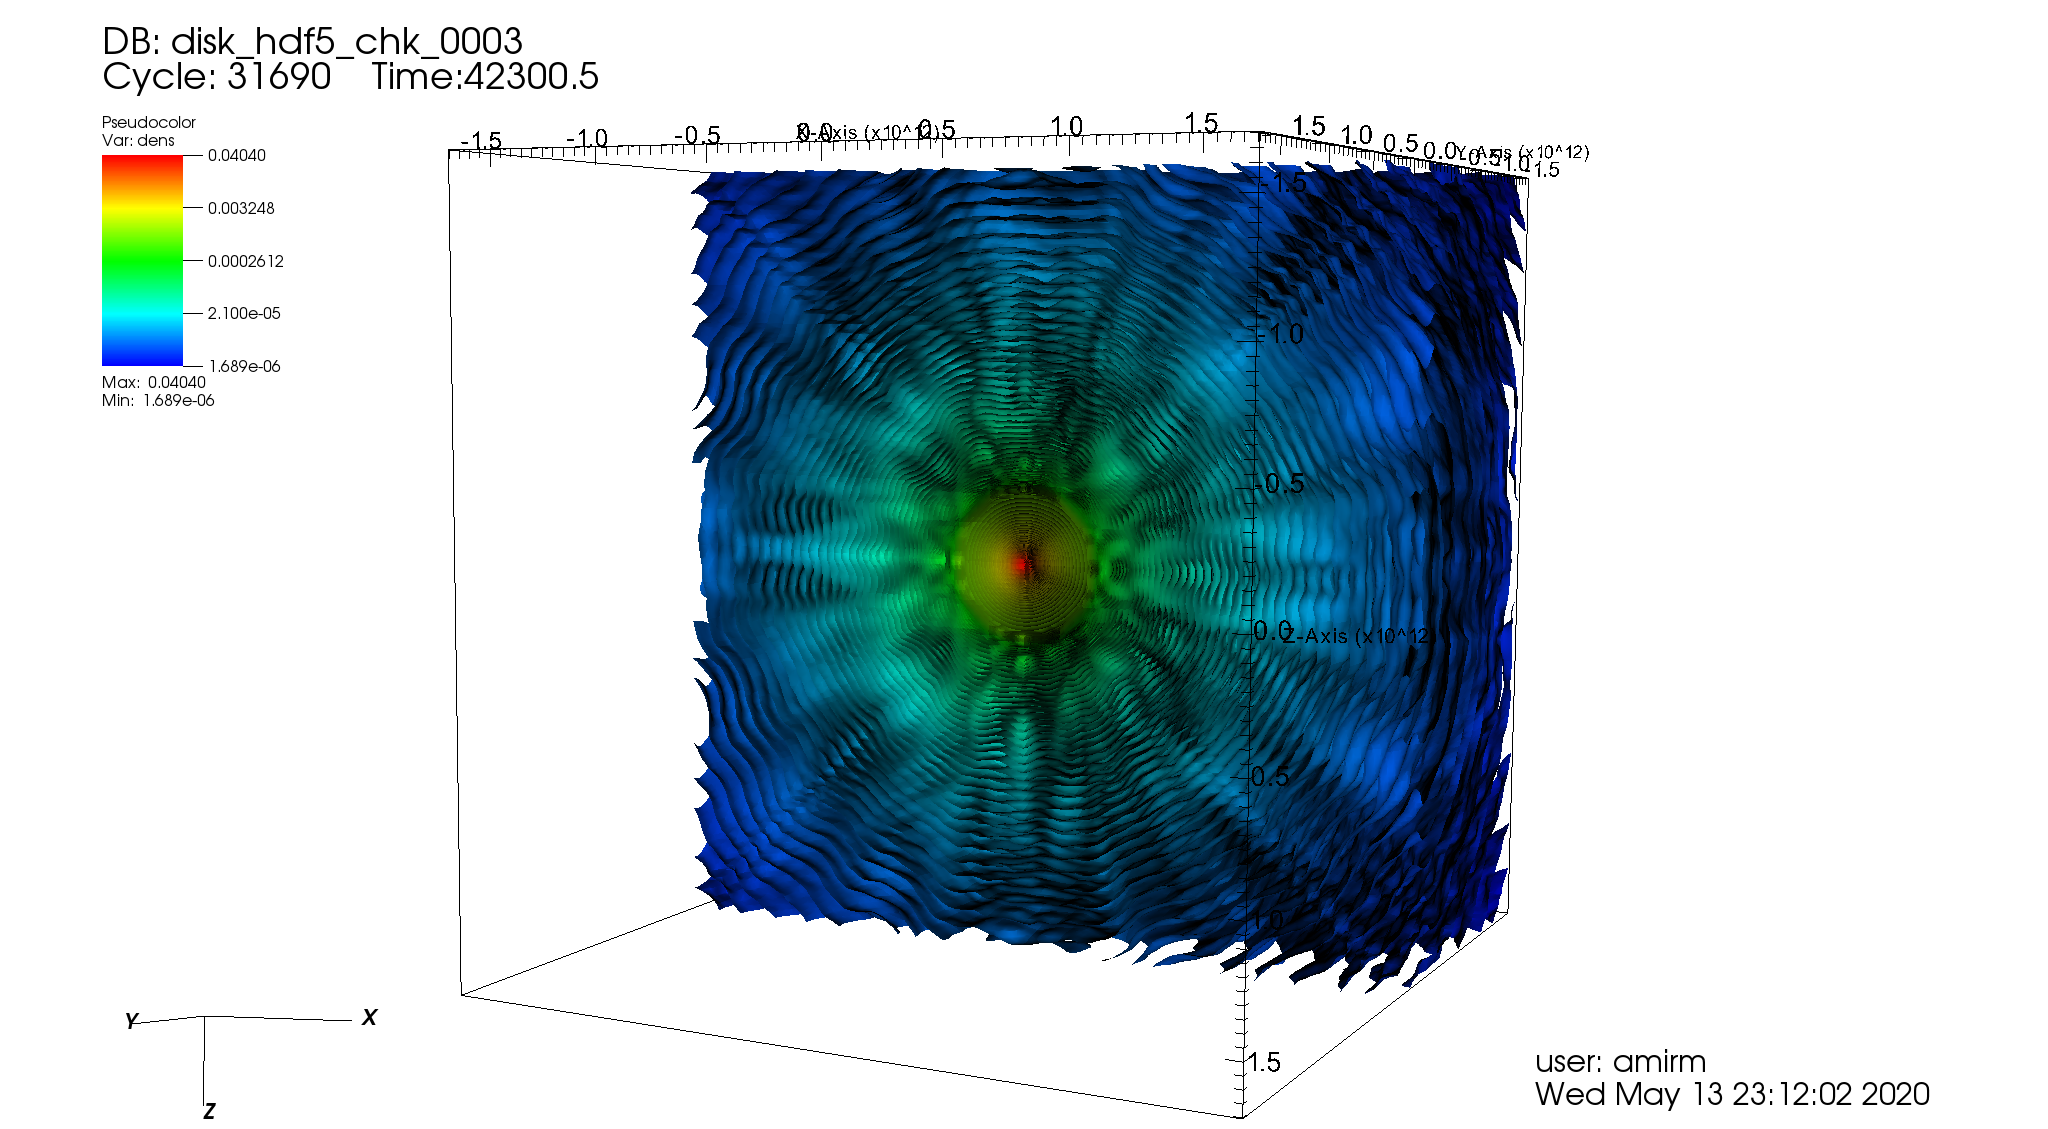
\includegraphics[width=1.0\textwidth]{density-3d-11-75.png}
    \end{center}
    \caption{
        The density 3D isosurface clip after 5:45 hours (simulation time) and 11:45 hours (simulation time).
    }\label{fig:dens-3d-t5-t11}
\end{figure}

\begin{figure}[ht!]
    \begin{center}
        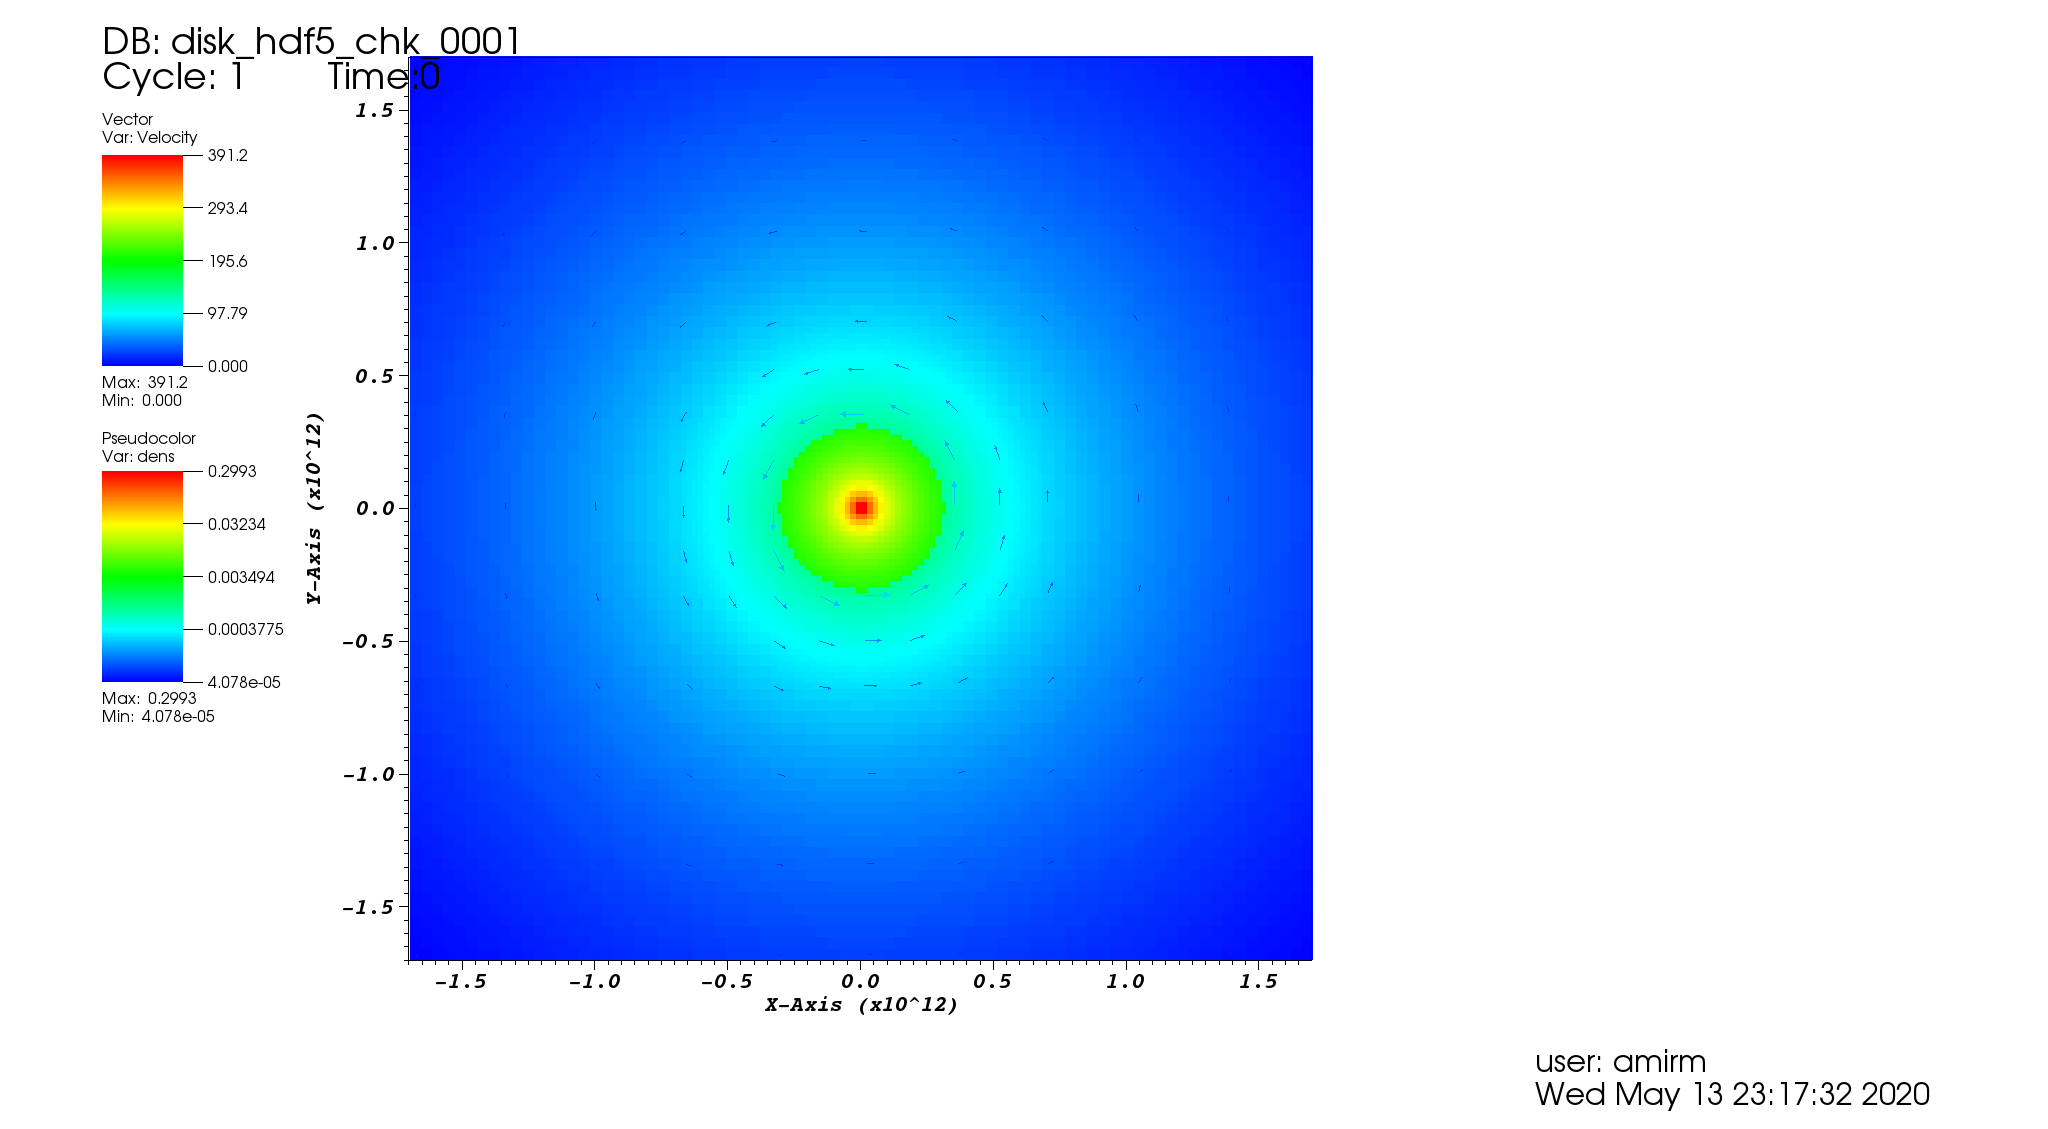
\includegraphics[width=0.8\textwidth]{density-vel-x-y-0.png}
        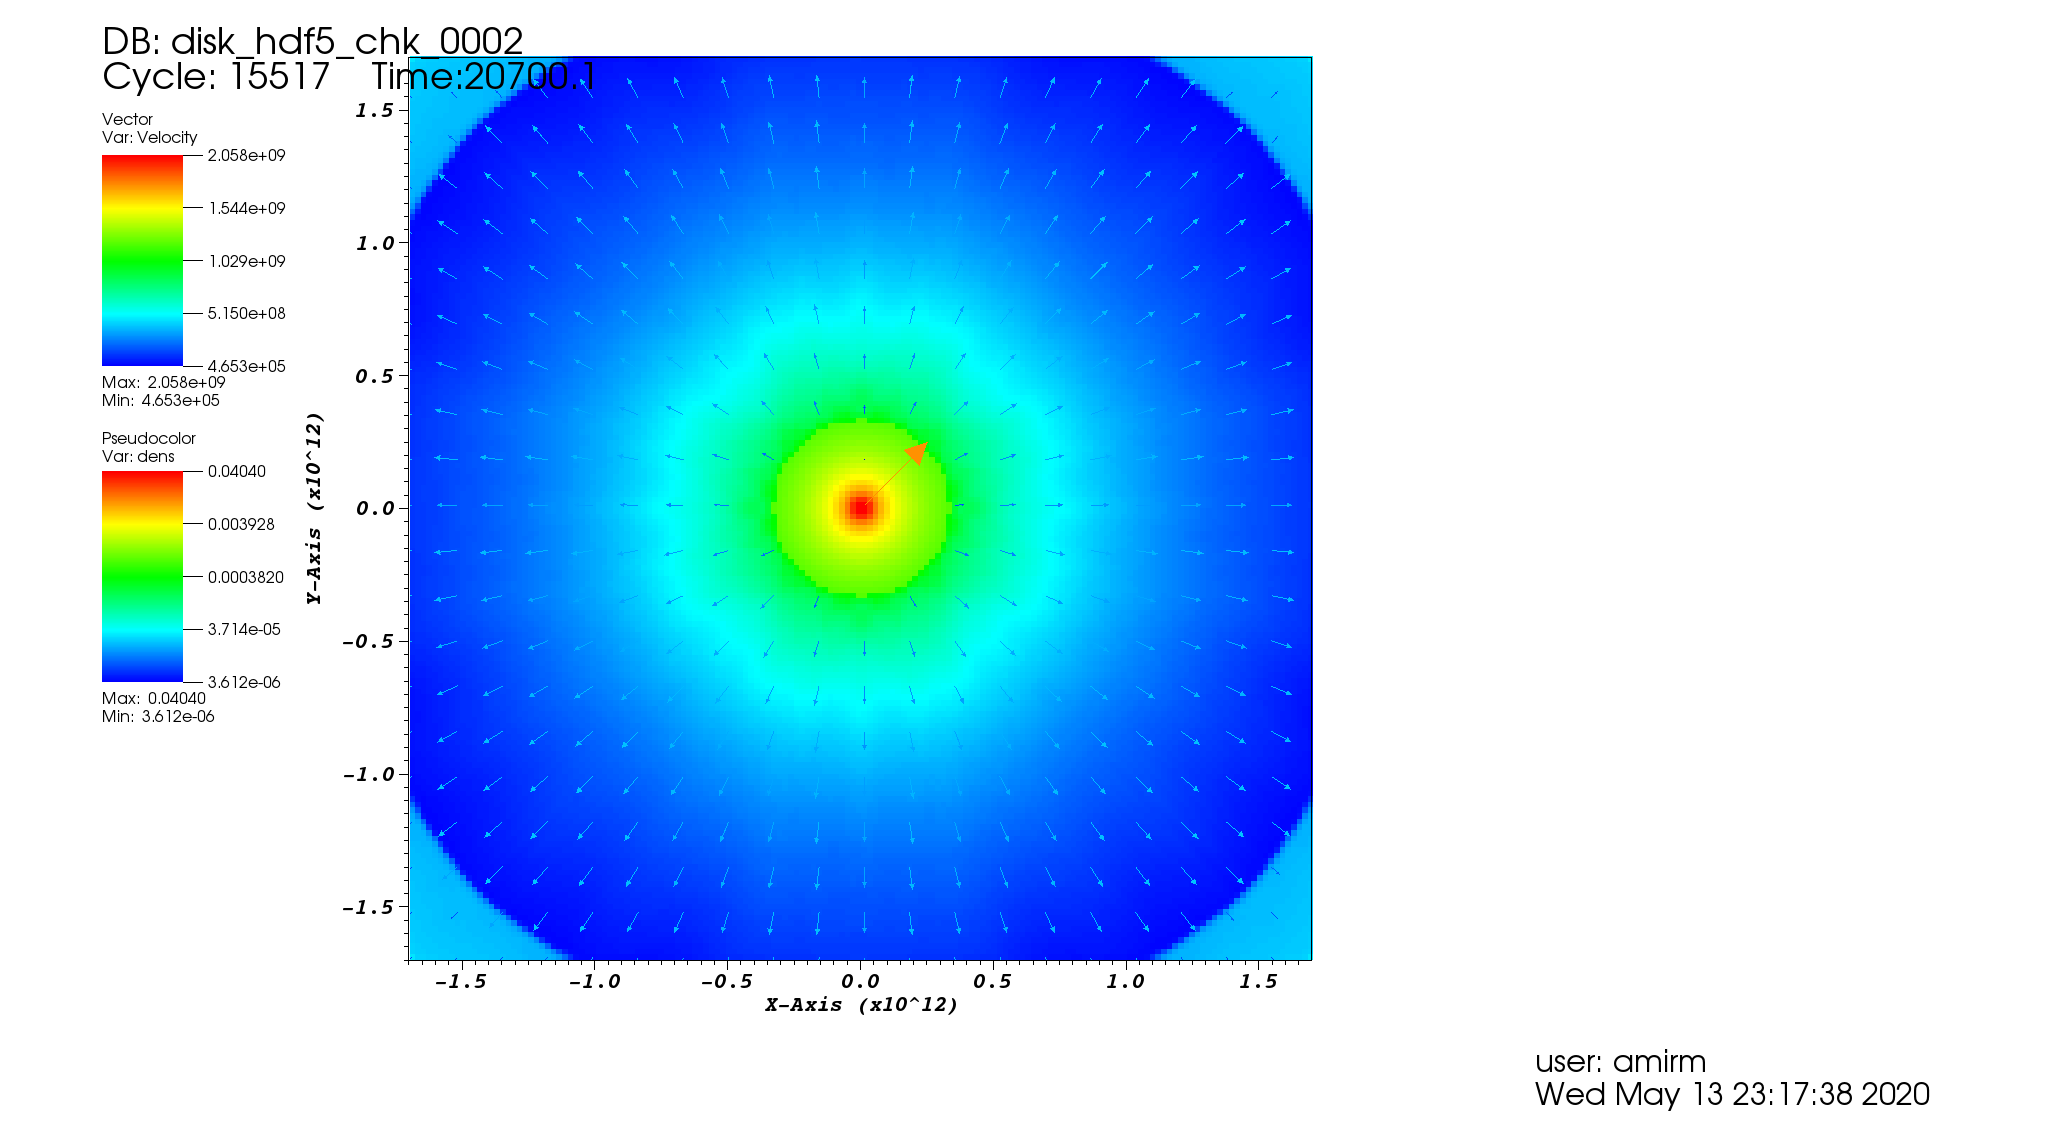
\includegraphics[width=0.8\textwidth]{density-vel-x-y-5-75.png}
        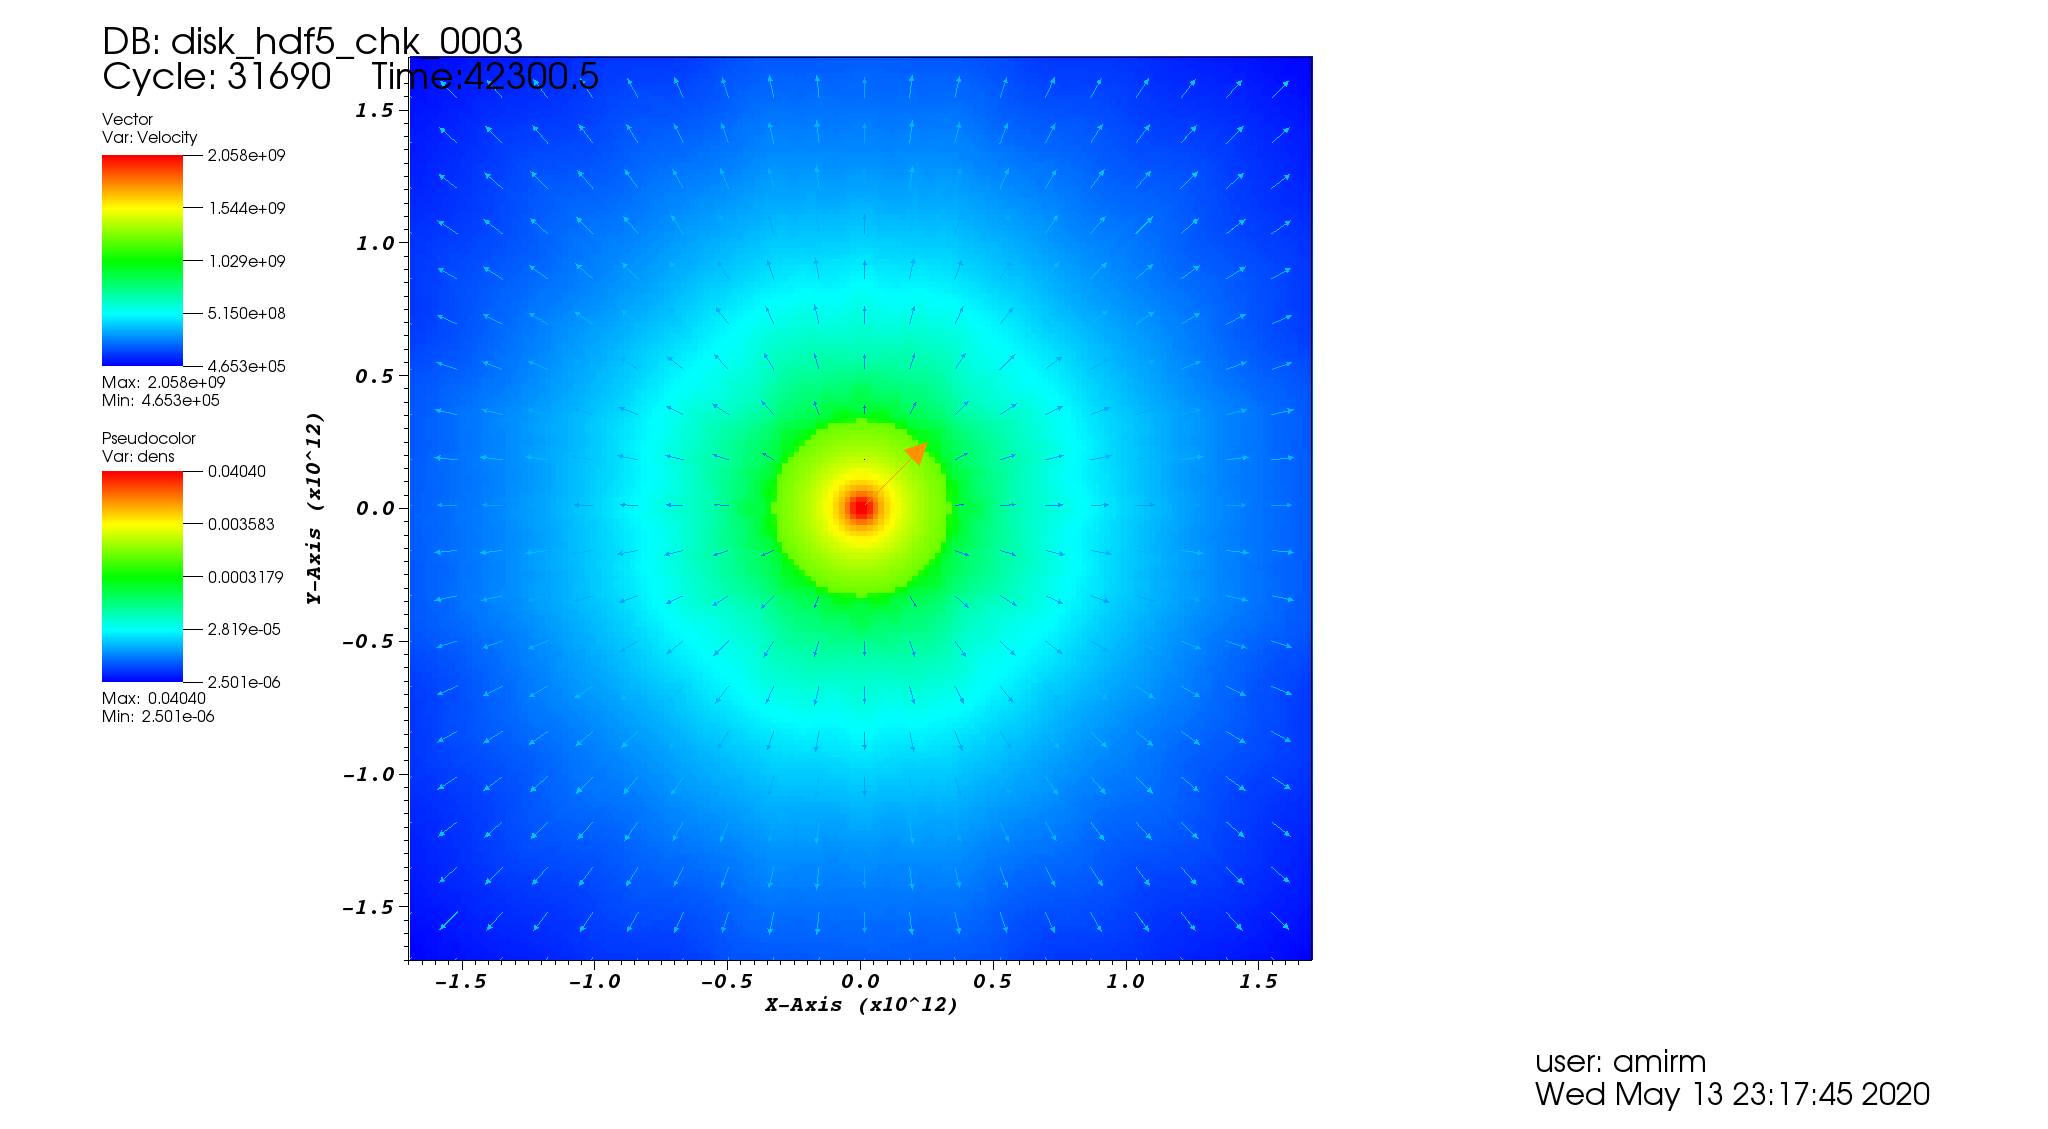
\includegraphics[width=0.8\textwidth]{density-vel-x-y-11-75.png}
    \end{center}
    \caption{
        x-y plane density and velocity at the start, after 5:45 hours (simulation time) and 11:45 hours (simulation time).
    }\label{fig:dens-vel-xy-t5-t11}
\end{figure}

%the problem and suggested solution.
The simulation take to long time.
As we can see there is a problem.
It seems there is to much matter in the unbound region out side the disk.
This suggested we need to change eq. \ref{eq:rho_outside_disk}.

Still working on that \dots

\bibliography{main}

\end{document} 
